\documentclass[11pt,a4paper]{article}
\usepackage[utf8]{inputenc}
\usepackage[french]{babel}
\usepackage[T1]{fontenc}

\usepackage{amsmath}
\usepackage{amsfonts}
\usepackage{amssymb}

\newcommand{\TitreMatiere}{Algorithmique : Premiers Pas}
\newcommand{\TitreSeance}{Notions de Bases}
\newcommand{\NumeroTD}{Bases d'Algorithmique}
\newcommand{\DateCours}{Septembre 2022}
\newcommand{\AnneeScolaire}{2022-2023}
\newcommand{\Organisation}{EPITA}
\newcommand{\NomAuteurA}{Fabrice BOISSIER}
\newcommand{\MailAuteurA}{fabrice.boissier@epita.fr}
\newcommand{\NomAuteurB}{ }
\newcommand{\MailAuteurB}{ }
\newcommand{\DocKeywords}{Algorithmique}
\newcommand{\DocLangue}{fr} % "en", "fr", ...

\usepackage{MetalQuickLabs}

% Babel ne traduit pas toujours bien les tableaux et autres
\renewcommand*\frenchfigurename{%
    {\scshape Figure}%
}
\renewcommand*\frenchtablename{%
    {\scshape Tableau}%
}

% Ne pas afficher le numéro de la légende sur tableaux et figures
\captionsetup{format=sanslabel}


\begin{document}

\EncadreTitre

\bigskip


%\begin{center}
%\begin{tabular}{p{5cm} p{11cm}}
%\textbf{Commandes étudiées :} & \texttt{sh}, \texttt{bash}, \texttt{man}, \texttt{ls}, \texttt{mkdir}, \texttt{touch}, \texttt{chmod}, \texttt{mv}, \texttt{rm}, \texttt{rmdir}, \texttt{cat}, \texttt{file}, \texttt{which}, \texttt{which}\\
%
%\textbf{Builtins étudiées :} & \texttt{pwd}, \texttt{cd}, \texttt{exit}, \texttt{logout}, \texttt{echo}, \texttt{umask}, \texttt{type}, \texttt{>}, \texttt{>{}>}, \texttt{<}, \texttt{<{}<}, \texttt{|}\\
%
%\textbf{Notions étudiées :} & Shell, Manuels, Fichiers, Répertoires, Droits, Redirections\\
%\end{tabular}
%\end{center}

\bigskip


Ce document a pour objectif de vous familiariser avec l'algorithmique.
Les tous premiers algorithmes que vous allez exécuter et écrire sont issus de connaissances communes vues lors de vos cours de l'enseignement primaire ou secondaire.

Pour exécuter les algorithmes en mode dit \textit{pas à pas}, pensez à toujours avoir une feuille de brouillon et un stylo pour pouvoir noter le déroulé de l'algorithme à chaque instruction ou série d'instructions.

\bigskip

Définition informelle d'un algorithme~\footnote{Introduction à l'Algorithmique. 2001 ($2^{e}$ édition) T.Cormen et al.} : \og \textit{procédure de calcul bien définie qui prend en entrée une valeur, ou un ensemble de valeurs, et qui donne en sortie une valeur, ou un ensemble de valeurs. Un algorithme est donc une séquence d'étapes de calcul qui transforment l'entrée en sortie} \fg .

\bigskip

%%%%%%%%%%%%%%%%%%%%%%%%%%%%%%%%%%%%%%

\section{Problèmes, Solutions, et Types de données}

\bigskip

Les algorithmes sont donc des étapes successives permettant d'obtenir un résultat.
Il s'agit littéralement de \textit{comment} traiter un problème pour pouvoir le résoudre.
Néanmoins, cette séquence d'étapes seule ne permet pas de savoir quel problème on souhaite traiter, il faut donc bien indiquer le contexte et l'objectif de l'algorithme.
Ainsi, le problème à traiter, le \textit{pourquoi}, est également extrêmement important.

\medskip

Chercher et comprendre les problèmes rencontrés est donc très important pour pouvoir écrire les algorithmes les plus efficaces.
Par exemple, si l'on cherche à trier des pierres selon leur taille, on utilisera des tamis de plus en plus large successivement pour récupérer tout d'abord les grains de sable, puis les cailloux les plus petits, et en dernier les pierres de plus grande taille (si l'on utilisait un tamis trop grand dès le début, toutes les tailles passeraient sans distinction).
Dans cet exemple, il était nécessaire de constater que la taille des pierres était très importante, que des outils permettent de laisser passer ou non des pierres d'une certaine taille sont disponibles, et que l'on ne s'intéressait finalement pas à d'immenses rochers.
Pour reprendre la comparaison avec les questions, les pierres et leurs tailles correspondent aux réponses du \textit{quoi}.
Ainsi :
\begin{itemize}
\item Pourquoi / Quel est l'objectif ? \textbf{Trier} des pierres par taille
\item Quoi / Que manipule-t-on ? Des pierres de différentes tailles
\item Comment ? En utilisant successivement des tamis avec des trous de plus en plus grands
\end{itemize}

\medskip

Ces spécifications seront très importantes lorsque vous serez amenés à écrire des algorithmes : pensez toujours à bien vérifier les \textit{spécifications} du problème avant d'essayer de répondre au problème (il peut arriver qu'en fait il n'y ait aucun problème).

\bigskip

En algorithmique, il existe quelques types fondamentaux permettant de représenter la plupart des informations du monde physique.
En combinant ces types, on peut donc représenter quasiment tout ce qui existe et est mesurable (la taille d'une pierre, sa composition chimique, sa dureté, sa brillance et sa forme une fois taillée, etc).

\begin{itemize}
\item entier (\textit{integer} en anglais) : il s'agit des entiers relatifs (positifs et négatifs)
\item flottant (\textit{float} ou \textit{double} en anglais) : il s'agit des nombres à virgule (attention, ce type a des problèmes de \textit{précision} : on ne peut pas toujours comparer correctement des flottants)
\item caractère (\textit{character} en anglais) : il s'agit des lettres ou caractères (à noter que ce type manipule une seule et unique lettre à la fois)
\item chaîne de caractères (\textit{string} en anglais) : il s'agit d'une suite de caractères
\end{itemize}

\bigskip

\newpage

%%%%%%%%%%%%%%%%%%%%%%%%%%%%%%%%%%%%%%

\section{Exécution pas à pas}

\bigskip

\question{Afin de bien comprendre comment fonctionne un algorithme, comment l'exécuter, et potentiellement comment le corriger, utilisez cet algorithme calculant la somme des $ n $ premiers entiers en l'exécutant à la main et en remplissant le tableau suivant pour $ n = 5 $.}

\begin{center}
\begin{equation*}
\sum^{n}_{i = 1} i = 1 + 2 + 3 + \ldots + n
\end{equation*}
\end{center}


\vfillFirst


%\begin{center}
%\begin{lstlisting}[style=sh,morekeywords={floor,ceil}]
%python
%\end{lstlisting}
%\end{center}

\begin{table}[!ht]
  \centering
  \begin{minipage}{0.59\textwidth}
    \centering
%    \begin{verbatim}
% %*   *)
\begin{lstlisting}[style=algorithmique]
algorithme fonction Somme : entier
  parametres locaux
    entier    n
  variables
    entier    i, sum

debut
i %*$\leftarrow$*) 1
sum %*$\leftarrow$*) 0
tant que (i <= n) faire
  sum %*$\leftarrow$*) sum + i
  i %*$\leftarrow$*) i + 1
fin tant que
retourne sum
fin algorithme fonction Somme \end{lstlisting}
%    \end{verbatim}
    % \caption{Algorithme de la somme des N premiers entiers}
    % \label{algo-somme-n-premiers-entiers}
  \end{minipage}
  \hfillx
  \begin{minipage}{0.4\textwidth}
    \centering
%    \begin{tabular}{|c|c|c|c|}
%        \hline
%        tour &  i &  sum  \\
%        \hline
%        0    &  1 &  0  \\
%        1    &  2 &  1  \\
%        2    &  3 &  3  \\
%        3    &  4 &  6  \\
%        4    &  5 & 10  \\
%        5    &  6 & 15  \\
%        \hline
%    \end{tabular}
    \begin{tabular}{|C{1cm}|C{1cm}|C{1cm}|}
        \hline
        tour &  i &  sum  \\
        \hline
             &    &       \\
        0    &    &       \\
             &    &       \\
        \hline
             &    &       \\
        1    &    &       \\
             &    &       \\
        \hline
             &    &       \\
        2    &    &       \\
             &    &       \\
        \hline
             &    &       \\
        3    &    &       \\
             &    &       \\
        \hline
             &    &       \\
        4    &    &       \\
             &    &       \\
        \hline
             &    &       \\
        5    &    &       \\
             &    &       \\
        \hline
             &    &       \\
        6    &    &       \\
             &    &       \\
        \hline
    \end{tabular}
    % \caption{Tableau d'exécution pas à pas}
    % \label{table-somme-n-premiers-entiers-execution}
  \end{minipage}
  \caption{Algorithme de la somme des N premiers entiers}
  \label{somme-n-premiers-entiers}
\end{table}


\vfillLast

\newpage

\vfillFirst


Reprenez maintenant l'exemple de la multiplication égyptienne en l'exécutant cette fois-ci à la main en remplissant le tableau suivant.

\question{Vous prendrez comme premières valeurs de test : $ a = 4 $ et $ b = 5 $.}

\question{Remplissez un tableau similaire sur un brouillon pour les valeurs $ a = 3 $ et $ b = 13 $.}

\bigskip

\begin{table}[h!]
  \centering
  \begin{minipage}{0.59\textwidth}
    \centering
%    \begin{verbatim}
% %*   *)
\begin{lstlisting}[style=algorithmique]
algorithme fonction MultEgpytienne : entier
  parametres locaux
    entier    a
    entier    b
  variables
    entier    x, y, z

debut
x %*$\leftarrow$*) a
y %*$\leftarrow$*) b
z %*$\leftarrow$*) 0
tant que (y > 0) faire
  si (y EST IMPAIRE) alors
     z %*$\leftarrow$*) z + x
  fin si
  x %*$\leftarrow$*) 2 %*×*) x
  y %*$\leftarrow$*) y %*÷*) 2
fin tant que
retourne z
fin algorithme fonction MultEgpytienne \end{lstlisting}
%    \end{verbatim}
    % \caption{Algorithme de la multiplication égyptienne}
    % \label{algo-multiplication-egyptienne}
  \end{minipage}
  \hfillx
  \begin{minipage}{0.4\textwidth}
    \centering
%    \begin{tabular}{|c|c|c|c|}
%        \hline
%        tour &  x &  y &  z  \\
%        \hline
%        0    &  4 &  5 &  0  \\
%        1    &  8 &  2 &  4  \\
%        2    & 16 &  1 &  4  \\
%        3    & 32 &  0 & 20  \\
%        \hline
%    \end{tabular}
    \begin{tabular}{|C{1cm}|C{1cm}|C{1cm}|C{1cm}|}
        \hline
        tour &  x &  y &  z  \\
        \hline
             &    &    &   \\
        0    &    &    &     \\
             &    &    &   \\
        \hline
             &    &    &   \\
        1    &    &    &     \\
             &    &    &   \\
        \hline
             &    &    &   \\
        2    &    &    &     \\
             &    &    &   \\
        \hline
             &    &    &   \\
        3    &    &    &     \\
             &    &    &   \\
        \hline
    \end{tabular}
    % \caption{Tableau d'exécution pas à pas}
    % \label{table-multiplication-egyptienne-execution}
  \end{minipage}
  \caption{Algorithme de la multiplication égyptienne}
  \label{multiplication-egyptienne}
\end{table}

%\bigskip
%
%    \begin{tabular}{|c|c|c|c|}
%        \hline
%        tour &  x &  y &  z  \\
%        \hline
%        0    &  3 & 13 &  0  \\
%        1    &  6 &  6 &  3  \\
%        2    & 12 &  3 &  3  \\
%        3    & 24 &  1 & 15  \\
%        3    & 48 &  0 & 39  \\
%        \hline
%    \end{tabular}

\bigskip


Dans le domaine informatique, on appelle \textit{traces d'exécution} le résultat d'exécution des programmes, avec si possible l'affichage de l'évolution de certaines variables et résultats.
En remplissant à la main les tableaux avec l'évolution des valeurs, vous avez produit des traces d'exécution.

Vous l'aurez compris, les traces sont beaucoup plus utiles lorsqu'il y a beaucoup de valeurs intéressantes suivies (il faut donc que les développeurs prévoient l'affichage de ces valeurs, ou une option permettant d'afficher ces traces).

En anglais, l'activation des options ou modes \textit{verbose} (qui pourrait être traduit par \textit{verbeux}) impliquent d'afficher un peu plus de variables qu'initialement prévu.
Ces affichages se font généralement dans des \textit{logs} (traduit par \textit{journaux}) ou à minima une sortie spécifique aux traces d'exécution pour ne pas les mélanger avec les résultats du comportement normal.


\vfillLast

\newpage

\vfillFirst


Effectuez maintenant l'algorithme de la division euclidienne.
L'algorithme renverra le quotient.

\question{Vous prendrez comme premières valeurs de test : $ a = 19 $ et $ b = 3 $.}

\bigskip

\begin{table}[h!]
  \centering
  \begin{minipage}{0.59\textwidth}
    \centering
%    \begin{verbatim}
% %*   *)
\begin{lstlisting}[style=algorithmique]
algorithme fonction DivEuclideQuotient : entier
  parametres locaux
    entier    a
    entier    b
  variables
    entier    x, y

debut
x %*$\leftarrow$*) a
y %*$\leftarrow$*) 0
tant que (x > 0) faire
  x %*$\leftarrow$*) x - b
  y %*$\leftarrow$*) y + 1
fin tant que
retourne y
fin algorithme fonction DivEuclideQuotient \end{lstlisting}
%    \end{verbatim}
    % \caption{Algorithme du quotient de la division euclidienne}
    % \label{algo-division-euclidienne-quotient}
  \end{minipage}
  \hfillx
  \begin{minipage}{0.4\textwidth}
    \centering
%    \begin{tabular}{|c|c|c|c|}
%        \hline
%        tour &  x &  y  \\
%        \hline
%        0    &  19 & 0  \\
%        1    &  16 & 1  \\
%        2    &  13 & 2  \\
%        3    &  10 & 3  \\
%        4    &   7 & 4  \\
%        5    &   4 & 5  \\
%        6    &   1 & 6  \\
%        \hline
%    \end{tabular}
    \begin{tabular}{|C{1cm}|C{1cm}|C{1cm}|}
        \hline
        tour &  x &   y   \\
        \hline
             &    &       \\
        0    &    &       \\
             &    &       \\
        \hline
             &    &       \\
        1    &    &       \\
             &    &       \\
        \hline
             &    &       \\
        2    &    &       \\
             &    &       \\
        \hline
             &    &       \\
        3    &    &       \\
             &    &       \\
        \hline
             &    &       \\
        4    &    &       \\
             &    &       \\
        \hline
             &    &       \\
        5    &    &       \\
             &    &       \\
        \hline
             &    &       \\
        6    &    &       \\
             &    &       \\
        \hline
    \end{tabular}
    % \caption{Tableau d'exécution pas à pas}
    % \label{table-division-euclidienne-quotient-execution}
  \end{minipage}
  \caption{Algorithme du quotient de la division euclidienne}
  \label{division-euclidienne-quotient}
\end{table}

\bigskip

\question{Quelle variable faut-il renvoyer pour obtenir le reste ?}

\bigskip

\question{Si le test dans le \textit{tant que} était un $ >= $ plutôt qu'un $ > $ : quels changements à l'exécution cela produirait-il ?}

\question{Quelles modifications faudrait-il apporter pour obtenir le bon quotient ? le bon reste ?}

\bigskip

\question{Cet algorithme est incapable de gérer le cas où $ 0 $ est fourni en tant que diviseur.
Comment pourrait-on corriger cela afin de protéger l'algorithme d'une boucle infinie ?}

\bigskip

Dans la plupart des langages de programmation, vous verrez qu'un opérateur \TTBF{mod} ou \TTBF{\%} existe et est assez fréquemment utilisée.
Il s'agit simplement de l'opérateur calculant le reste de la division euclidienne.

$ 42 \; \% \; 10 = 2 $ (lorsque l'on divise $ 42 $ par $ 10 $, le reste est $ 2 $)

$ 40 \; \% \; 10 = 0 $ (lorsque l'on divise $ 40 $ par $ 10 $, le reste est $ 0 $)

$ 42 \; \% \; 2 = 0 $ (lorsque l'on divise $ 42 $ par $ 2 $, le reste est $ 0 $)

$ 9 \; \% \; 10 = 9 $ (lorsque l'on divise $ 9 $ par $ 10 $, le reste est $ 9 $)


\vfillLast

\newpage

%%%%%%%%%%%%%%%%%%%%%%%%%%%%%%%%%%%%%%

\section{\'Ecriture d'algorithmes simples}

\bigskip

Plusieurs opérations qui nous semblent évidentes sont en réalité bien plus complexes à réaliser dans la pratique.

La multiplication égyptienne est un exemple très concret de cela : nous savons multiplier car nous avons appris et compris ce qu'il se passait lors de cette opération, mais sans l'apprentissage, il est difficile de connaitre le résultat d'une multiplication.
Tout comme il est difficile de multiplier de tête des nombres à virgules entre eux.

Les opérations simples sont cependant essentielles à l'écriture de programmes et d'algorithmes plus complexes.

\bigskip

\vspace*{3cm}

\bigskip

\question{Maintenant que vous savez lire, exécuter (y compris en mode pas à pas), et corriger un algorithme, écrivez l'algorithme de la multiplication classique à base d'additions ($ N \text{×} M = $ N additions de la valeur M) dans le cas de nombres positifs uniquement.}

\bigskip

\vspace*{0.5cm}

\bigskip

N'hésitez pas à utiliser un exemple général simple pour bien déterminer la boucle à écrire :
\begin{center}

$ 5 \text{×} 3 = 5 + 5 + 5 = 15 $

\end{center}

\bigskip

On peut donc s'attendre à avoir une accumulation dans une variable pour le résultat :
\begin{center}

$ 0, 5, 10, 15 $

\bigskip

$ 0 (+ 5) $

$ 5 (+ 5) $

$ 10 (+ 5) $

$ 15 $
\end{center}

\bigskip

Mais, on doit également connaître le cas d'arrêt : lorsque le multiplicateur est à $ 0 $.


\begin{center}
\begin{tabular}{|C{1cm}|C{1cm}|C{1cm}|}
 \hline
  5 & 3 &  0 \\
  5 & 2 &  5 \\
  5 & 1 & 10 \\
  5 & 0 & 15 \\
 \hline
\end{tabular}
\end{center}


%\bigskip
\newpage

\vfillFirst

\begin{table}[ht!]
  \centering
  \begin{minipage}{0.59\textwidth}
    \centering
% %*   *)
\begin{lstlisting}[style=algorithmique]

algorithme fonction MultClassique : entier
  parametres locaux
    entier    a
    entier    b
  variables
    entier

debut










fin algorithme fonction MultClassique
 \end{lstlisting}
  \end{minipage}
  \hfillx
  \begin{minipage}{0.4\textwidth}
    \centering
%    \begin{tabular}{|c|c|c|c|}
%        \hline
%        tour &  i &   j &  k  \\
%        \hline
%        0    &  1 &   1 &   0 \\
%        1    &  2 &   1 &   1 \\
%        2    &  3 &   2 &   3 \\
%        3    &  4 &   6 &   9 \\
%        4    &  5 &  24 &  33 \\
%        5    &  6 & 120 & 153 \\
%        \hline
%    \end{tabular}
    \begin{tabular}{|C{1cm}|C{1cm}|C{1cm}|C{1cm}|}
        \hline
             &     &     &     \\
        \hline
             &     &     &   \\
             &     &     &     \\
             &     &     &   \\
        \hline
             &     &     &   \\
             &     &     &     \\
             &     &     &   \\
        \hline
             &     &     &   \\
             &     &     &     \\
             &     &     &   \\
        \hline
             &     &     &   \\
             &     &     &     \\
             &     &     &   \\
        \hline
             &     &     &   \\
             &     &     &     \\
             &     &     &   \\
        \hline
    \end{tabular}
  \end{minipage}
%  \caption{Multiplication classique}
%  \label{multiplication-classique}
\end{table}

\bigskip

\question{Comment peut-on traiter les nombres négatifs ? Écrivez maintenant une fonction \textit{MultRelatifs} permettant de multiplier des nombres entiers négatifs (n'hésitez pas à appeler la fonction de multiplication que vous avez précédemment écrite).}


\vfillLast

\newpage

\vfillFirst


\question{Écrivez l'algorithme calculant la puissance de $ x^{n} $ (pour $ n $ positif ou nul).}

Au lieu d'utiliser les symbole × ou * pour multiplier, vous ferez un appel à votre dernière fonction \textit{MultRelatifs} en lui donnant deux paramètres et en récupérant le résultat.

\bigskip


\begin{table}[ht!]
  \centering
  \begin{minipage}{0.59\textwidth}
    \centering
% %*   *)
\begin{lstlisting}[style=algorithmique]

algorithme fonction Puissance : entier
  parametres locaux
    entier    a
    entier    b
  variables
    entier

debut

















fin algorithme fonction Puissance
 \end{lstlisting}
  \end{minipage}
  \hfillx
  \begin{minipage}{0.4\textwidth}
    \centering
%    \begin{tabular}{|c|c|c|c|}
%        \hline
%        tour &  i &   j &  k  \\
%        \hline
%        0    &  1 &   1 &   0 \\
%        1    &  2 &   1 &   1 \\
%        2    &  3 &   2 &   3 \\
%        3    &  4 &   6 &   9 \\
%        4    &  5 &  24 &  33 \\
%        5    &  6 & 120 & 153 \\
%        \hline
%    \end{tabular}
    \begin{tabular}{|C{1cm}|C{1cm}|C{1cm}|C{1cm}|}
        \hline
             &     &     &     \\
        \hline
             &     &     &   \\
             &     &     &     \\
             &     &     &   \\
        \hline
             &     &     &   \\
             &     &     &     \\
             &     &     &   \\
        \hline
             &     &     &   \\
             &     &     &     \\
             &     &     &   \\
        \hline
             &     &     &   \\
             &     &     &     \\
             &     &     &   \\
        \hline
             &     &     &   \\
             &     &     &     \\
             &     &     &   \\
        \hline
    \end{tabular}
  \end{minipage}
%  \caption{Puissance}
%  \label{puissance}
\end{table}

\vfillLast


\newpage


\vfillFirst

\question{Écrivez l'algorithme testant la parité d'un nombre $ n $.}

La parité est simplement la qualité d'un nombre d'être pair ou impair.
Vous renverrez $ 0 $ en cas de nombre pair, et $ 1 $ en cas de nombre impair.

\bigskip


\begin{center}

% %*   *)
\begin{lstlisting}[style=algorithmique]

algorithme fonction Parite : entier
  parametres locaux
    entier    n
  variables
    entier

debut










fin algorithme fonction Parite
\end{lstlisting}

\end{center}


\vfillLast

\newpage

%%%%%%%%%%%%%%%%%%%%%%%%%%%%%%%%%%%%%%

\section{Logique et écriture d'algorithmes}

\bigskip

En mathématiques, un domaine étudie en particulier la \textit{logique} de façon formelle (logique de premier ordre, ...).
Ce domaine est directement appliqué en électronique numérique avec les portes logiques (\textit{logic gates} en anglais) et les bascules (\textit{flip-flops} en anglais).

\medskip

La logique s'appuie sur deux valeurs qui s'opposent : \TTBF{vrai} (1) et \TTBF{faux} (0).
Il est possible d'exprimer des assertions avec des \textit{formules logiques} afin de vérifier si celles-ci sont vraies ou fausses dans certains cas selon des paramètres.
Pour cela, plusieurs opérateurs logiques existent.
Les trois opérateurs fondamentaux (faisant découler toute une série d'autres opérateurs utiles) existent : \TTBF{NOT} (non), \TTBF{AND} (et), \TTBF{OR} (ou).

\medskip

\TTBF{NOT} est un opérateur unaire, il ne s'applique qu'à un seul paramètre : \og - A \fg{}.

\TTBF{AND} et \TTBF{OR} sont des opérateurs binaires, ils s'appliquent à deux paramètres : \og A et B \fg{}, \og A ou B \fg{}.

Nous représentons dans les tableaux suivants ce qui s'appelle des \textit{tables de vérités} : les résultats des assertions logiques.

\bigskip

\begin{table}[ht!]
    \centering
    \hfill
    \begin{tabular}{|c|c|}
        \hline
        A & \TTBF{NOT} \tabularnewline
        \hline
        0 & 1 \tabularnewline
        \hline
        1 & 0 \tabularnewline
        \hline
    \end{tabular}
    \hfill
    \begin{tabular}{|c|c|c|}
        \hline
        A & B & \TTBF{AND} \\
        \hline
        0 & 0 & 0 \\
        \hline
        0 & 1 & 0 \\
        \hline
        1 & 0 & 0 \\
        \hline
        1 & 1 & 1 \\
        \hline
    \end{tabular}
    \hfill
    \begin{tabular}{|c|c|c|}
        \hline
        A & B & \TTBF{OR} \\
        \hline
        0 & 0 & 0 \\
        \hline
        0 & 1 & 1 \\
        \hline
        1 & 0 & 1 \\
        \hline
        1 & 1 & 1 \\
        \hline
    \end{tabular}
    \hfill\null
\end{table}

\bigskip

Ces trois opérateurs sont très souvent utilisés pour tester des conditions.
Si le résultat est vrai ($ 1 $), alors la condition est validée.
On peut combiner ces opérateurs pour tester des assertions logiques.

\bigskip

Cependant, ces opérateurs sont également appliqués dans le cadre de langages de programmation pour modifier des valeurs au niveau des bits les constituant (comme nous le verrons plus tard).
En plus de \TTBF{NOT}, \TTBF{OR}, \TTBF{AND}, vous pourrez rencontrer les opérateurs \TTBF{NAND} (non et), \TTBF{NOR} (non ou), et le très important \TTBF{XOR} (ou exclusif) qui est extrêmement utilisé en cryptographie.
Ces opérateurs sont simplement des combinaisons des trois opérateurs fondamentaux : \TTBF{NAND} applique simplement un \TTBF{NOT} au résultat du \TTBF{AND}, et \TTBF{NOR} applique simplement un \TTBF{NOT} au résultat du \TTBF{OR}.

\TTBF{XOR} est légèrement plus complexe dans sa construction, mais sa logique est simple : il faut que les deux entrées soient dans des état différents pour que le résultat soit vrai ($ 1 $).
Vous pouvez néanmoins constater qu'en appliquant un \TTBF{AND} aux sorties de \TTBF{OR} et \TTBF{NAND}, on obtient la même table de vérité.

\bigskip

\begin{table}[ht!]
    \centering
    \hfill
    \begin{tabular}{|c|c|c|}
        \hline
        A & B & \TTBF{NAND} \\
        \hline
        0 & 0 & 1 \\
        \hline
        0 & 1 & 1 \\
        \hline
        1 & 0 & 1 \\
        \hline
        1 & 1 & 0 \\
        \hline
    \end{tabular}
    \hfill
    \begin{tabular}{|c|c|c|}
        \hline
        A & B & \TTBF{NOR} \\
        \hline
        0 & 0 & 1 \\
        \hline
        0 & 1 & 0 \\
        \hline
        1 & 0 & 0 \\
        \hline
        1 & 1 & 0 \\
        \hline
    \end{tabular}
    \hfill
    \begin{tabular}{|c|c|c|}
        \hline
        A & B & \TTBF{XOR} \\
        \hline
        0 & 0 & 0 \\
        \hline
        0 & 1 & 1 \\
        \hline
        1 & 0 & 1 \\
        \hline
        1 & 1 & 0 \\
        \hline
    \end{tabular}
    \hfill\null
\end{table}

\bigskip

%Dans les programmes que vous développez, vous utiliserez régulièrement des conditions pour vérifier des assertions.
%Cependant, il existe un autre usage que la vérification de condition pour les opérateurs booléens précédemment présentés.
%Lorsque l'on représente des valeurs numériques dans un ordinateur avec des bits, on peut appliquer les opérateurs booléens dessus et modifier la valeur représentée.

%%%%%%%%%%%%%%%%%%%%%%%%%%%%%%%%%%%%%%%%%%%%%%%%%%%%%%%%%%%%%%%%%%%%%%%%%%%%%%%%%%%%%%%%%%%%%%%%%%%%%%%%%%%

\subsection{Exercices de logique}

\question{Écrivez une fonction prenant 3 entiers en paramètre, et indiquant lequel est le plus petit/grand. \textit{min(a, b, c) max(a, b, c)} }


\newpage

%%%%%%%%%%%%%%%%%%%%%%%%%%%%%%%%%%%%%%

\section{Récursivité}

\bigskip

La récursivité est un principe très simple où une fonction se rappelle elle-même. %, comme lorsque l'on effectue une boucle et qu'une variable évolue petit à petit.

\smallskip

L'écriture d'algorithmes récursifs implique au moins deux choses dans cet ordre très précis : une condition d'arrêt où l'on retourne le résultat, puis, un appel récursif avec un paramètre modifié (si on ne modifie aucun paramètre, alors la récursion serait infinie : on rappellerait la fonction dans les mêmes conditions qu'actuellement, donc elle se rappellerait encore une fois avec strictement les mêmes paramètres).

\smallskip

Il est nécessaire d'écrire les conditions d'arrêts en premier, car il s'agit des cas exceptionnels où l'on doit arrêter la récursion.
De même, il est hautement conseillé d'écrire les cas les plus génériques en dernier, car des cas partiellement exceptionnels pourraient être absorbés plus tôt par le cas général.
Par exemple, si l'on souhaite dénombrer les N premiers entiers, et afficher à chaque dizaine un message particulier, on déclarera en premier la condition d'arrêt où un paramètre est à $ 0 $ ou $ 1 $, puis, on écrira la condition testant les valeurs notables particulières (ici si le paramètre est une dizaine), et en tout dernier on écrira le cas général qui concerne n'importe quelle valeur.

\bigskip


\subsection{Exercices récursifs}

Maintenant que vous avez écrit quelques algorithmes simples avec des boucles, nous allons passer à leurs versions récursives.

\bigskip

\question{Commencez par exécuter l'algorithme de la somme des N premiers entiers en remplissant le tableau avec l'évolution des paramètres donnés dans un premier temps, puis des résultats. Vous effectuerez cette exécution avec $ 5 $ comme paramètre.}

\bigskip

\begin{table}[h!]
  \centering
  \begin{minipage}{0.5\textwidth}
    \centering
%    \begin{verbatim}
% %*   *)
\begin{lstlisting}[style=algorithmique]
algorithme fonction SommeRec : entier
  parametres locaux
    entier    n

debut
si (n == 1) alors
  retourne (1)
sinon
  retourne (n + SommeRec(n - 1))
fin si
fin algorithme fonction SommeRec \end{lstlisting}
%    \end{verbatim}
    % \caption{Algorithme de la somme des N premiers entiers}
    % \label{algo-somme-n-premiers-entiers-recursif}
  \end{minipage}
  \hfillx
  \begin{minipage}{0.13\textwidth}
    \centering
    \begin{tabular}{|C{1cm}|C{1cm}|}
        \hline
        appel &  n  \\
        \hline
              &     \\
        0     &     \\
              &     \\
        \hline
              &     \\
        1     &     \\
              &     \\
        \hline
              &     \\
        2     &     \\
              &     \\
        \hline
              &     \\
        3     &     \\
              &     \\
        \hline
              &     \\
        4     &     \\
              &     \\
        \hline
              &     \\
        5     &     \\
              &     \\
        \hline
              &     \\
        6     &     \\
              &     \\
        \hline
    \end{tabular}
    % \caption{Tableau d'appels}
    % \label{table-somme-n-premiers-entiers-appels}
  \end{minipage}
  \hfillx
  \begin{minipage}{0.24\textwidth}
    \centering
    \begin{tabular}{|C{1cm}|C{1cm}|C{1cm}|}
        \hline
        appel & retour & total \\
        \hline
              &        & \\
        6     &        & \\
              &        & \\
        \hline
              &        & \\
        5     &        & \\
              &        & \\
        \hline
              &        & \\
        4     &        & \\
              &        & \\
        \hline
              &        & \\
        3     &        & \\
              &        & \\
        \hline
              &        & \\
        2     &        & \\
              &        & \\
        \hline
              &        & \\
        1     &        & \\
              &        & \\
        \hline
              &        & \\
        0     &        & \\
              &        & \\
        \hline
    \end{tabular}
    % \caption{Tableau de retours}
    % \label{table-somme-n-premiers-entiers-retours}
  \end{minipage}
  \caption{Somme des N premiers entiers (récursif)}
  \label{somme-n-premiers-entiers-recursif}
\end{table}


\bigskip

Vous remarquerez que l'algorithme est beaucoup plus court en quantité d'instructions.
Ceci est principalement dû au fait que le calcul que nous exécutons est déjà dans une forme adaptée (souvenez-vous du principe de récurrence, ou encore des suites) : la même opération est répétée avec un paramètre réduit ou augmenté de $ 1 $ (ou d'un pas bien défini).

\bigskip

\question{Écrivez maintenant l'algorithme de la factorielle, mais de façon récursive. N'oubliez pas : on écrit d'abord la ou les conditions d'arrêt, et ensuite seulement on effectue l'opération avec l'appel récursif.}

\begin{equation*}
  \begin{aligned}
& n! = 1 \times 2 \times 3 \times \ldots \times n
  \end{aligned}
\end{equation*}

\bigskip

\question{Écrivez l'algorithme récursif calculant la somme des N premiers entiers.}

\begin{equation*}
  \begin{aligned}
& \sum^{n}_{i = 1} i = 1 + 2 + 3 + \ldots + n
  \end{aligned}
\end{equation*}

\bigskip

\question{Écrivez l'algorithme récursif calculant la multiplication de deux entiers positifs, en n'utilisant que des additions et des soustractions.}

\question{Améliorez l'algorithme de la multiplication pour qu'elle gère maintenant les nombres négatifs. Vous pouvez pour cela vous aider d'une fonction chapeau, c'est-à-dire une fonction qui prend les deux paramètres attendus (les deux nombres à multiplier) et fait différents tests avant d'appeler une autre fonction qui elle sera récursive.}

\bigskip

\question{Écrivez l'algorithme récursif calculant le Nième terme d'une suite géométrique. Vous devriez avoir en paramètres : le terme $ u_{0} $ désignant le premier terme de la suite, la raison $ q $, et le numéro $ n $ du terme recherché.}

\begin{equation*}
  \begin{aligned}
& u_{n} = u_{0} \times q^{n}
  \end{aligned}
\end{equation*}

\bigskip

\question{Écrivez une fonction récursive calculant le $ n^{\text{ème}} $ terme de la suite de Fibonacci.}

\begin{equation*}
  \begin{aligned}
& fibo(0) = fibo(1) = 1 \\
& fibo(n) = fibo(n - 1) + fibo(n - 2)
  \end{aligned}
\end{equation*}

\question{Écrivez maintenant la version itérative de la suite de Fibonacci. [Astuce : on dispose de deux cas à valeurs fixes, et à chaque étape on doit se rappeler du résultat précédent.] }

\bigskip

\question{Écrivez une fonction récursive calculant le $ n^{\text{ème}} $ terme de la suite d'Ackermann.}

\begin{equation*}
  \begin{aligned}
& A(0, n) = n + 1                 &  [n >= 0] & \\
& A(m, 0) = A(m - 1, 1)           &  [m > 0]  & \\
& A(m, n) = A(m - 1, A(m, n - 1)) &  [m > 0 \; \& \; n > 0] &
  \end{aligned}
\end{equation*}

\bigskip

\question{Écrivez l'algorithme récursif calculant le nombre de combinaisons de $ p $ dans $ n $ ($ C^{p}_{n} $ ou CPN), c'est-à-dire le nombre de parties à $ p $ éléments dans un ensemble $ E $ contenant $ n $ éléments.}

\bigskip

Par exemple : pour $ p = 2 $, on recherche tous les \textbf{couples} possibles de différents éléments.
Pour $ p = 3 $, on recherche tous les \textbf{triplets} possibles de différents éléments.
En indiquant $ n = 3 $, on vise un ensemble composé de trois éléments distincts (par exemple : $ E = \{ 1, 2, 3 \} $, ou $ E = \{ A, B, C \} $, ou $ E = \{ \spadesuit, \heartsuit, \clubsuit \} $, il s'agit juste de trois éléments distincts).

%\bigskip
\newpage

Ainsi, pour $ p = 2 $ et $ n = 3 $, on recherche tous les couples possibles de trois éléments :

\begin{table}[h!]
  \centering
  \begin{tabular}{l l}
(A,B) & (A,C) \\
      & (B,C)
  \end{tabular}
\end{table}

\hspace*{3cm} $\Rightarrow$ $ C^{2}_{3} = 3 $ \hspace*{1cm} (3 couples possibles)

\bigskip

Pour $ p = 2 $ et $ n = 4 $, on recherche tous les couples possibles de quatre éléments :

\begin{table}[h!]
  \centering
  \begin{tabular}{l l l}
(A,B) & (A,C) & (A,D) \\
      & (B,C) & (B,D) \\
      &       & (C,D)
  \end{tabular}
\end{table}

\hspace*{3cm} $\Rightarrow$ $ C^{2}_{4} = 6 $ \hspace*{1cm} (6 couples possibles)

\bigskip

Pour $ p = 3 $ et $ n = 3 $, on recherche tous les triplets possibles de trois éléments :

\begin{table}[h!]
  \centering
  \begin{tabular}{l}
(A,B,C) \\
  \end{tabular}
\end{table}

\hspace*{3cm} $\Rightarrow$ $ C^{3}_{3} = 1 $ \hspace*{1cm} (1 triplet possible)

\bigskip

Pour $ p = 3 $ et $ n = 4 $, on recherche tous les triplets possibles de quatre éléments :

\begin{table}[h!]
  \centering
  \begin{tabular}{l l l}
(A,B,C) & (A,B,D) & (A,C,D) \\
        &         & (B,C,D) \\
  \end{tabular}
\end{table}

\hspace*{3cm} $\Rightarrow$ $ C^{3}_{4} = 4 $ \hspace*{1cm} (4 triplets possibles)

\bigskip

Voici les axiomes pour votre implémentation :

\begin{table}[h!]
  \centering
  \begin{tabular}{l l}
$ C(0,n) = 1 $                             & \\
$ C(n,n) = 1 $                             & $ [n \neq 0] $ \\
$ C(p,n) = C(p, n - 1) + C(p - 1, n - 1) $ & $ [n \neq p] $ \\
  \end{tabular}
\end{table}


\clearpage

%%%%%%%%%%%%%%%%%%%%%%%%%%%%%%%%%%%%%%

\subsection{Exercices variés (récursif \& itératif)}

\bigskip

Les exercices dans cette section doivent plutôt être réalisés en itératif.
Il est précisé lesquels peuvent aisément être réalisés en récursif.
Il est interdit d'utiliser les tableaux ou pointeurs pour réaliser ces exercices.

\bigskip

\question{Écrivez une fonction prenant 3 entiers en paramètre, et indiquant lequel est le plus petit/grand. \textit{min(a, b, c) max(a, b, c)} }

\bigskip

\question{Écrivez une fonction transformant un format horaire en un format uniquement composé de secondes. Cette fonction prendra 3 entiers en paramètre (les heures, les minutes, et les secondes) et les convertira en secondes. Par exemple, 1h 23m 45s deviendra 5025 secondes. \textit{ConversionHoraire1(hh, mm, ss)} }

\bigskip

\question{Écrivez une autre fonction de conversion horaire qui prend cette fois un unique entier qui respecte un format précis (hhmmss) pour le convertir en secondes. Par exemple le paramètre 153042 signifie 15h 30m 42s qu'il faut convertir en secondes. \textit{ConversionHoraire2(hhmmss)} }

\bigskip

\question{Écrivez une fonction qui transforme un nombre en son miroir. Cette fonction prend un entier en paramètre, et construit un autre entier qui est son miroir. Par exemple, pour 12034, son miroir sera 43021. Autre exemple : 2000 aura comme miroir 0002, c'est-à-dire 2. Attention aux nombres composés d'un nombre pair/impair de chiffres. Commencez par réaliser une fonction itérative. \textit{MiroirIter(n)} }

\bigskip

\question{Écrivez maintenant la version récursive du nombre miroir. Pour cette première version récursive, vous appelerez une fonction \textit{écrire(x)} ou \textit{print(x)} qui affiche un caractère ou un chiffre à la fois. \textit{MiroirRec1(n)} }

\bigskip

\question{Écrivez maintenant la version récursive du nombre miroir. Pour cette deuxième version récursive, vous devrez renvoyer le nombre miroir et non pas juste l'afficher. \textit{MiroirRec2(n)}}

Astuce : vous pouvez utiliser un \textit{accumulateur} comme deuxième paramètre, donc, écrire une fonction chapeau qui prendra un seul paramètre et préparera l'appel à la fonction récursive.

\bigskip

\question{Écrivez une fonction récursive qui affiche les éléments successifs de la conjecture de Syracuse, mais qui renvoie également le nombre d'éléments produits avant d'atteindre $ 1 $. Utilisez les fonctions \textit{écrire(x)} ou \textit{print(x)} et une fonction chapeau si nécessaire. \textit{Syracuse(n)} }

Voici les axiomes pour votre implémentation :

\begin{table}[h!]
  \centering
  \begin{tabular}{l l}
$ Syracuse(0) = 1 $       & \\
$ Syracuse(1) = 1 $       & \\
$ Syracuse(n) = n / 2 $   & si $ n $ est paire \\
$ Syracuse(n) = 3n + 1 $  & si $ n $ est impaire \\
  \end{tabular}
\end{table}

\question{Écrivez une fonction détectant si un nombre est un palindrome. La fonction renvoie \textit{vrai} si c'est un palindrome, sinon elle renvoie \textit{faux}. Un palindrome est simplement un mot ou un nombre composé des mêmes caractères ou chiffres sur sa première moitié par rapport à sa deuxième moitié. Par exemple, 27972 est un palindrome. 1331 est également un palindrome, mais 1664 n'en est pas un. Faites d'abord une version itérative, puis faites une version récursive. \textit{PalindromeIter(n)} \textit{PalindromeRec(n)} }

\newpage

%%%%%%%%%%%%%%%%%%%%%%%%%%%%%%%%%%%%%%

\section{Tableaux et Chaînes de caractères}

\bigskip

Les tableaux en algorithmique, et dans la plupart des langages de programmation, sont simplement des vecteurs.
C'est-à-dire qu'il s'agit de tableaux à une seule dimension.
La plupart des langages de programmation font démarrer leurs tableaux à la position $ 0 $.
Ceci implique qu'un tableau de taille $ 5 $ (donc qui contient $ 5 $ cases) démarre de la case $ 0 $ et finit à la case $ 4 $ ($ 0 1 2 3 4 $).
Dans vos algorithmes, vous manipulerez donc souvent les cases de $ 0 $ à \textit{longueur du tableau - 1}, avec comme condition \textit{tant que (iterateur < longueur)} (on s'arrête lorsque l'itérateur atteint la longueur, donc après la dernière case du tableau).
Il existe cependant quelques langages où les tableaux démarrent à la case $ 1 $, donc finissent à la case \textit{longueur du tableau} : vérifiez toujours quel est l'index (le numéro de case) de la première case dans chacun des langages de programmation que vous utiliserez.

\medskip

\begin{table}[h!]
  \centering
  \begin{tabular}{| c | c | c | c | c |}
  \hline
$ 42 $ & $ 14 $ & $ 18 $ & $ 666 $ & $ 1337 $ \\
  \hline
% 0    &   1    &    2   &    3    &    4     \\
\textit{0} & \textit{1} & \textit{2} & \textit{3} & \textit{4} \\
  \hline
  \end{tabular}
\end{table}

\medskip

Les tableaux contiennent parfois des éléments de types différents (des entiers, des flottants, et des chaînes de caractères), mais il est fréquent qu'ils ne peuvent contenir qu'un seul et unique type à la fois (uniquement des entiers, ou uniquement des flottants, ou uniquement un type précis).
Dans les exercices de ce sujet, nos tableaux ne pourront contenir qu'un seul et unique type à chaque fois.
Si vous déclarez un tableau d'entiers, alors on ne peut y mettre que des entiers et rien d'autre.

\bigskip

Pour accéder à une case précise d'un tableau, on indique l'index entre crochets.
Par exemple, pour un tableau d'entiers stocké dans la variable \textit{tab}, on accède à la première case en écrivant : \textit{tab[0]}.
On peut récupérer le contenu de la case pour le mettre dans une variable en écrivant \textit{var = tab[2]}.
On peut écrire une valeur dans une case d'un tableau en écrivant \textit{tab[2] = 42}.

\bigskip

L'index peut également être une variable, mais celle-ci doit être un entier (on ne peut pas accéder à une case dont l'index est un flottant ou un caractère).
Ainsi, on ne peut ni faire \textit{tab[0,42]} ni \textit{tab['a']} ni \textit{tab["trois"]}, mais si une variable $ n $ contient un entier (par exemple : $ n = 3 $), on peut écrire \textit{tab[n]}.

\bigskip

Toujours concernant les index des cases, si on essaye d'accéder à une case inexistante (par exemple un index négatif comme $ -1 $ ou au delà de la taille du tableau), une erreur est renvoyée.
Par exemple, pour un tableau de taille $ 5 $ (index de 0 à 4), on peut accéder à la case $ 4 $ (\textit{tab[4]}) mais pas à la case $ 5 $ (\textit{tab[5]}).

\bigskip

Les chaînes de caractères (c'est-à-dire les suites de caractères) sont en réalité des tableaux contenant des caractères.
Le format standard des chaînes de caractères implique qu'une chaîne finisse par un unique caractère spécial : '\textit{\textbackslash 0}'.
Ainsi, la chaîne de caractères standard "lol" est en réalité un tableau de taille $ 4 $ dont la dernière case contient '\textbackslash 0'.
Grâce à cette convention, on n'a plus besoin d'embarquer la taille de la chaîne, il suffit juste de chercher un '\textbackslash 0' pour comprendre qu'il n'y a rien après.

\bigskip

\begin{table}[h!]
  \centering
  \begin{tabular}{| c | c | c | c |}
  \hline
'l' & 'o' & 'l' & '\textbackslash 0' \\
  \hline
% 0  &  1  &  2  &  3 \\
\textit{0} & \textit{1} & \textit{2} & \textit{3} \\
  \hline
  \end{tabular}
\end{table}

\bigskip

Vous pouvez néanmoins rencontrer des chaînes de caractères non-standards, c'est-à-dire qu'elles ne finissent pas nécessairement par '\textbackslash 0', et peuvent même en contenir dans la chaîne elle-même.
Dans ce cas très précis, on vous fournira toujours la taille de la chaîne de caractère en plus du tableau.

\bigskip

\begin{table}[h!]
  \centering
  \begin{tabular}{| c | c | c | c | c | c | c |}
  \hline
'A' & 'b' & 'C' & '\textbackslash 0' & 'D' & 'e' & 'F' \\
  \hline
% 0  &  1  &  2  &          3         &  4  &  5  &  6  \\
\textit{0} & \textit{1} & \textit{2} & \textit{3} & \textit{4} & \textit{5} & \textit{6} \\
  \hline
  \end{tabular}
\end{table}

%\bigskip
\clearpage

\subsection{Exercices variés (tableaux)}

\question{Écrivez maintenant une fonction palindrome fonctionnant sur un tableau dont la longueur est donnée en paramètre. \textit{PalindromeTab(tab, len)} }

\bigskip

\question{Écrivez une fonction palindrome fonctionnant sur une chaîne de caractères (le '\textbackslash 0' final ne sera bien entendu pas pris en compte dans le palindrome). \textit{PalindromeStr(str)} }

\bigskip

\question{Écrivez une fonction comparant deux tableaux. Si les tableaux sont les mêmes, alors vous renverrez \textit{vrai}, sinon vous renverrez \textit{faux}. \textit{CompareTab(tab1, tab2, len1, len2)} }

\bigskip

\question{Écrivez une fonction qui renvoie la valeur la plus grande/petite du tableau. Vous ferez une version itérative et une version récursive pour Min et Max. \textit{MinTabIter(tab, len)} \textit{MaxTabIter(tab, len)} \textit{MinTabRec(tab, len)} \textit{MaxTabRec(tab, len)} }

\bigskip

\question{Écrivez une fonction qui calcule la somme de tous les éléments d'un tableau. Vous ferez une version itérative et une version récursive. \textit{SommeTabIter(tab, len)} \textit{SommeTabRec(tab, len)} }

Améliorez l'algorithme pour n'utiliser qu'un seul itérateur tout en ajoutant à chaque fois le début et la fin du tableau (n'oubliez pas de vous arrêter là où il faut et de ne pas ajouter trop d'éléments).

\bigskip

\question{Écrivez une fonction qui calcule la taille d'une chaîne de caractères (sans compter le '\textbackslash 0' final : "lol" a une taille de $ 3 $). Vous ferez une version itérative et une version récursive. \textit{StrlenIter(str)} \textit{StrlenRec(str)} }

\bigskip

\question{Écrivez une fonction qui compare deux chaînes de caractères et renvoie \textit{vrai} si elles sont similaires et \textit{faux} si elles diffèrent. Vous ferez une version itérative et une version récursive. \textit{StrcmpIter(str1, str2)} \textit{StrcmpRec(str1, str2)} }

Essayez d'écrire une version itérative qui teste d'abord la longueur des chaînes, puis, une autre version sans ce test.

\bigskip

\question{Écrivez une fonction qui recherche un élément dans un tableau. Vous ferez une version itérative et une version récursive. \textit{RechercheEltTabIter(tab, len, elt)} \textit{RechercheEltTabRec(tab, len, elt)} }

\bigskip

\question{Écrivez une fonction qui compare deux tableaux. Si les deux tableaux contiennent les mêmes éléments aux mêmes positions, vous renverrez \textit{vrai}, sinon vous renverrez \textit{faux}. Vous ferez une version itérative et une version récursive. \textit{CompareTabIter(tab1, tab2, len1, len2)} \textit{CompareTabRec(tab1, tab2, len1, len2)} }

\bigskip

\question{Écrivez une fonction qui teste si les éléments d'un tableau sont tous en ordre croissant. Si tous les éléments sont ordonnés du plus petit au plus grand, alors vous renverrez \textit{vrai}, sinon vous renverrez \textit{faux}. Si les éléments sont tous égaux, alors le résultat sera \textit{vrai}. Vous ferez une version itérative et une version récursive. \textit{TestCroissantTabIter(tab, len)} \textit{TestCroissantTabRec(tab, len)} }

Faites la même chose pour tester la décroissance.

\bigskip

\question{Écrivez une fonction qui insère un élément dans un tableau à une position précise, et décale les éléments vers la fin. Le dernier élément qui devrait disparaître du tableau sera renvoyé par la fonction. Par exemple, pour un tableau contenant [ A B C D ], si l'on y insère 'Z' en position $ 1 $, le tableau doit devenir [ A Z B C ] et la fonction doit renvoyer D. \textit{InsertionTab(tab, len, elt, pos)} }

\bigskip

\question{Écrivez une fonction qui supprime un élément dans un tableau à une position précise, et décale les éléments vers le début. L'élément supprimé du tableau sera renvoyé par la fonction. De plus, pour éviter que le dernier élément soit dupliqué, vous prendrez un élément en paramètre qui sera inséré à la fin. Par exemple, pour un tableau contenant [ A B C D ], si l'on supprime l'élément en position $ 1 $ tout en ajoutant 'Z', le tableau doit devenir [ A C D Z ] et la fonction doit renvoyer B. \textit{SuppressionTab(tab, len, pos, elt)} }

\bigskip

\question{Écrivez une procédure qui inverse la position de tous les éléments. Vous ne devez pas construire de nouveau tableau, mais uniquement modifier en place le tableau (en utilisant des variables temporaires). Par exemple, pour un tableau contenant [ A B C D ], si l'on inverse la position des éléments, le tableau doit devenir [ D C B A ]. \textit{InverserTab(tab, len)} }

\bigskip

\question{Écrivez une fonction qui vérifie sur une chaîne de caractères est bien un préfixe d'une autre chaîne de caractères. Cette fonction renvoie \textit{vrai} si le prefixe est bon et \textit{faux} si ce n'est pas le cas. Par exemple, "abc" est un préfixe à "abcdef", mais pas "bcd" ni "def". Vous ferez une version itérative et une version récursive. \textit{PrefixStrIter(str, prefix)} \textit{PrefixStrRec(str, prefix)} }

\bigskip

\question{Écrivez une fonction qui vérifie sur une chaîne de caractères est bien un suffixe d'une autre chaîne de caractères. Cette fonction renvoie \textit{vrai} si le suffixe est bon et \textit{faux} si ce n'est pas le cas. Par exemple, "def" est un suffixe à "abcdef", mais pas "cde" ni "abc". Vous ferez une version itérative et une version récursive. \textit{SuffixStrIter(str, suffix)} \textit{SuffixStrRec(str, suffix)} }

\bigskip

\question{Écrivez une fonction qui vérifie sur une chaîne de caractères est contenue dans une autre chaîne de caractères. Cette fonction renvoie \textit{vrai} si la sous-chaîne est contenue dans la chaîne principale et \textit{faux} si ce n'est pas le cas. Par exemple, "abc" est contenue dans "ababc", mais pas "cde" ni "cba". Vous ferez une version itérative et une version récursive. \textit{SubStrIter(str, sub)} \textit{SubStrRec(str, sub)} }

Attention, certains cas sont difficiles à détecter.
Dans certains cas, il sera plus difficile de détecter "abc" dans "abcbc" que "abc" dans "ababc".
N'oubliez pas de vérifier plusieurs cas complexes tels que : rechercher "abc" dans "abababc" ou "abcbcbc".


%\newpage

%%%%%%%%%%%%%%%%%%%%%%%%%%%%%%%%%%%%%%

\section{Tris}

\bigskip

\question{Écrivez une fonction qui inverse la position de deux éléments. Vous ne devez pas construire de nouveau tableau, mais uniquement modifier en place le tableau (en utilisant des variables temporaires). Par exemple, pour un tableau contenant [ A B C D ], si l'on inverse la position des éléments $ 0 $ et $ 1 $, le tableau doit devenir [ B A C D ]. \textit{SwapEltTab(tab, len, pos1, pos2)} }

\bigskip

\subsection{Tri à bulles}

\bigskip

Le tri à bulles vise à faire remonter tour à tour les plus grandes valeurs vers la fin du tableau.
Si deux valeurs côté à côté sont dans le désordre, on les inverse, et on teste les suivantes jusqu'à la fin du tableau.
Avec cette méthode, dès que l'on trouve la plus grande valeur du tableau, celle-ci avancera progressivement jusqu'à la fin.
Avant d'atteindre la plus grande valeur, on peut également faire remonter les autres valeurs plus grandes.
Cependant, à chaque fois que l'on parcourt intégralement le tableau de gauche à droite, on est sûr que la valeur la plus à droite est à sa place finale.
Ainsi, on réduit la zone à parcourir à chaque tour : une fois la plus grande valeur du tableau trouvée à la fin du premier tour et placée à la dernière case, on n'a plus besoin de chercher dans cette case (l'élément étant maintenant à sa place).

%\medskip
\clearpage

\vfillFirst

%\begin{figure*} % Figure flottante
\begin{figure}[ht!]
\centering
\centerline{
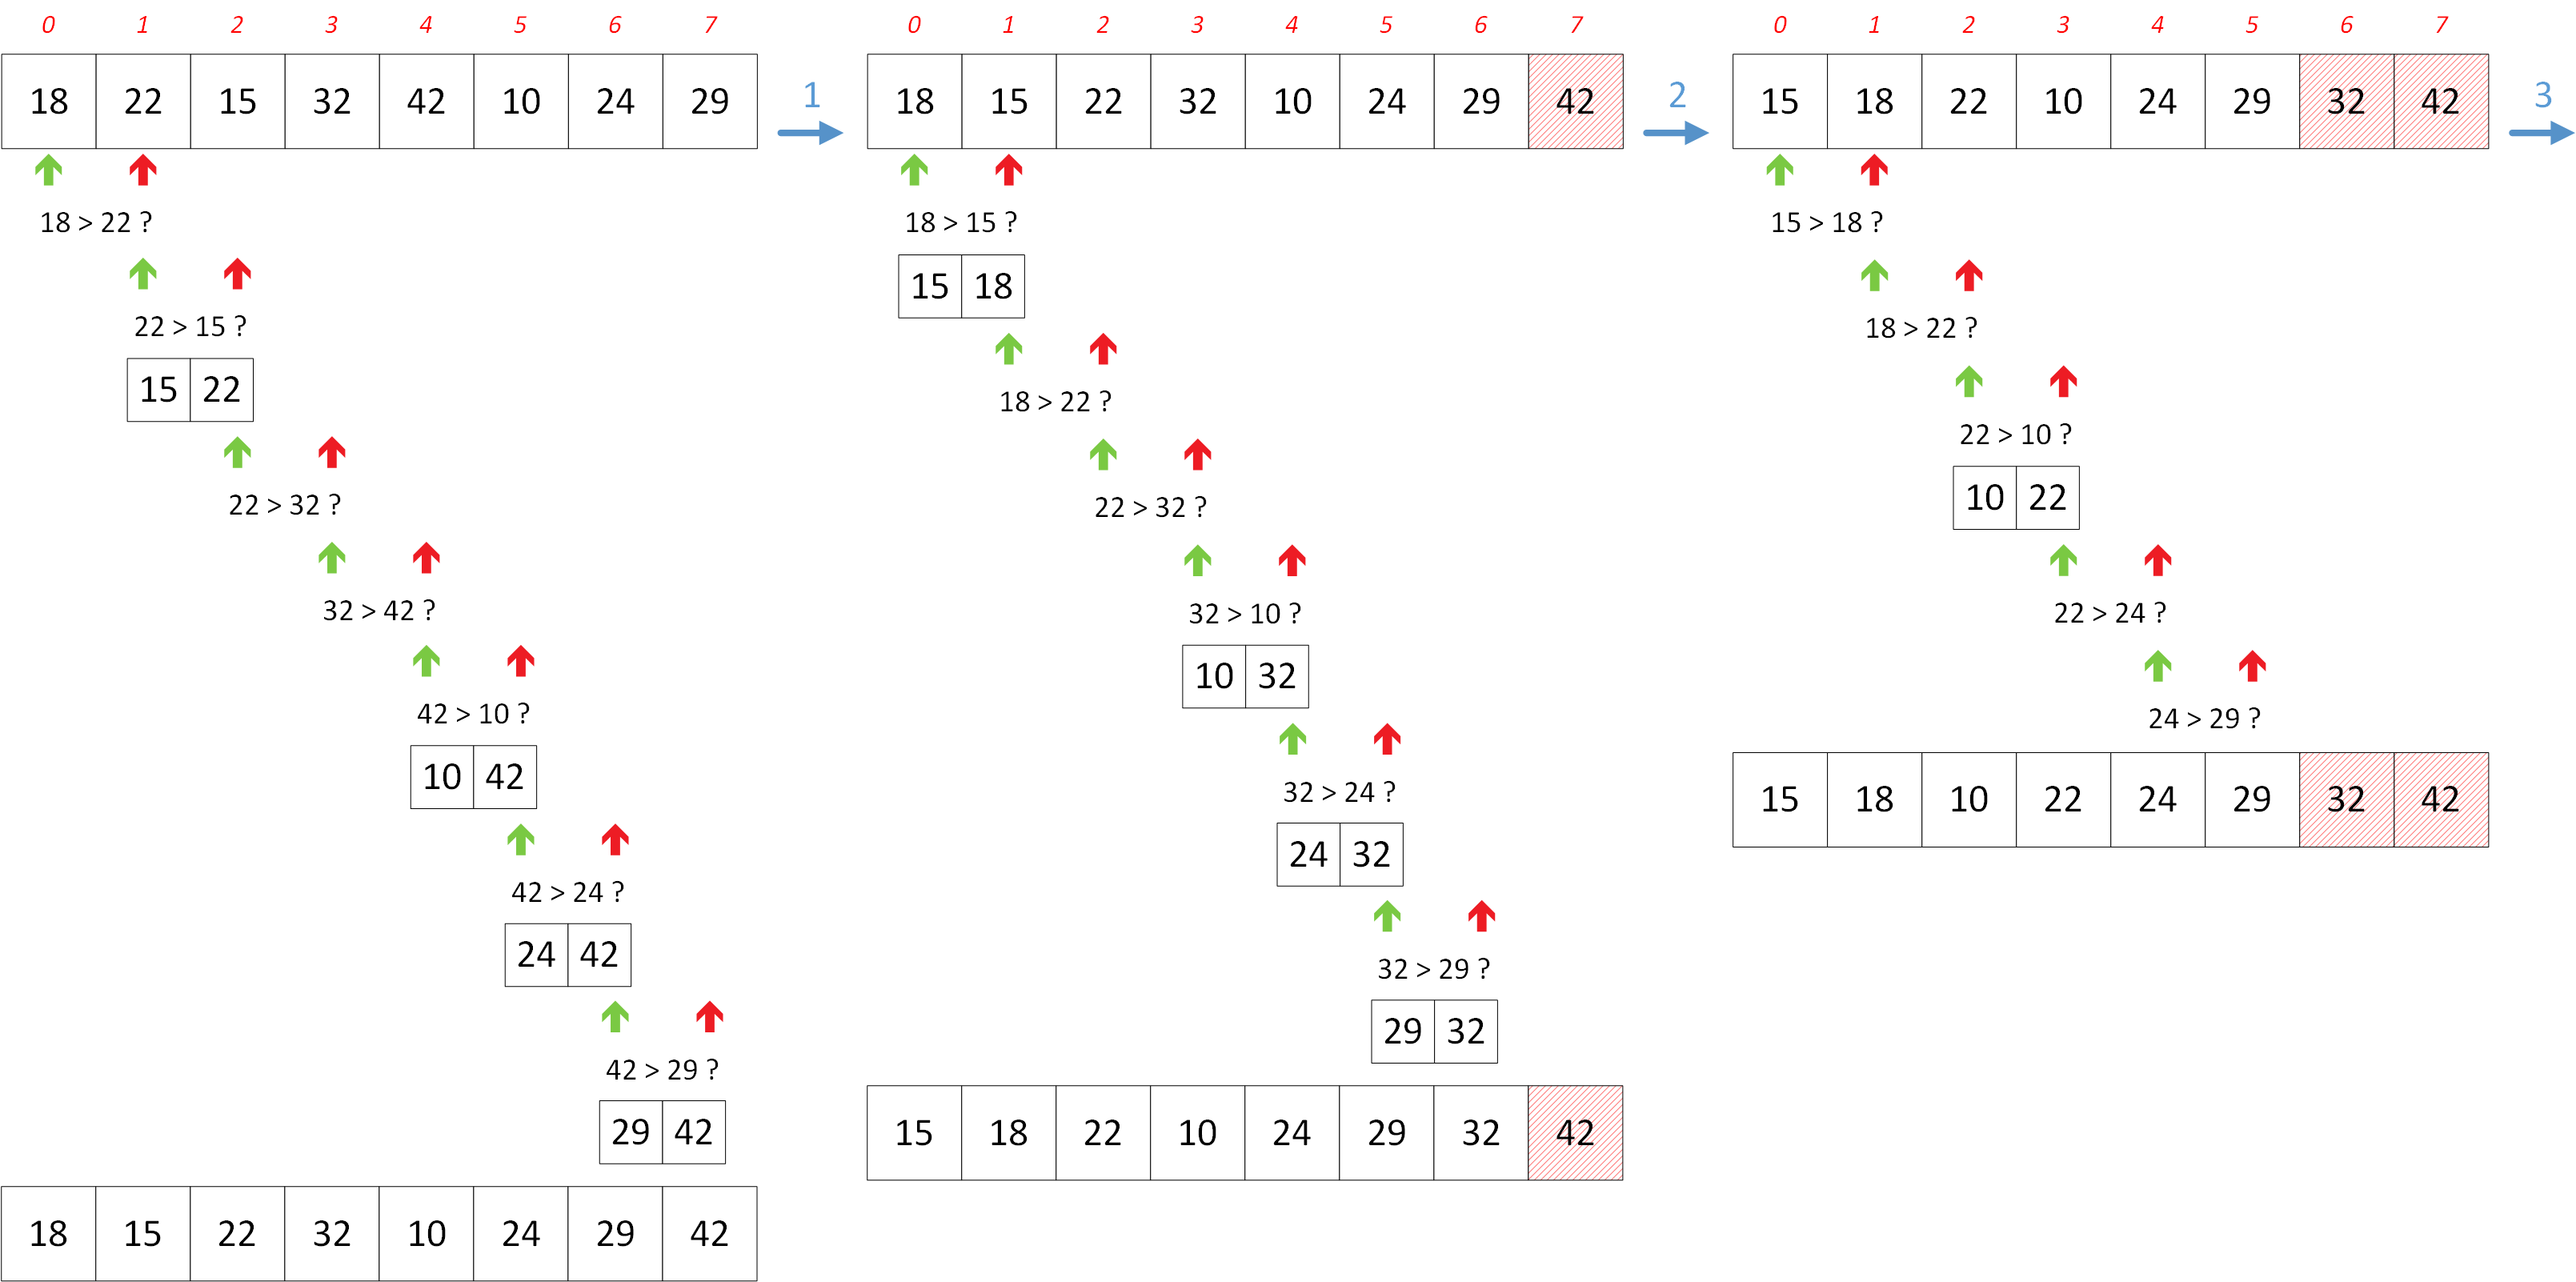
\includegraphics[width=1.2\textwidth]{img/BubbleSort_part1.png}
}
%\caption{Bubble Sort part 1}
%\label{figure:1-S3-DesignScience-ThreeLoops}
\end{figure}
%\end{figure*} % Figure flottante
% To use it : fig~\ref{label}

%\begin{figure*} % Figure flottante
\begin{figure}[ht!]
\centering
\centerline{
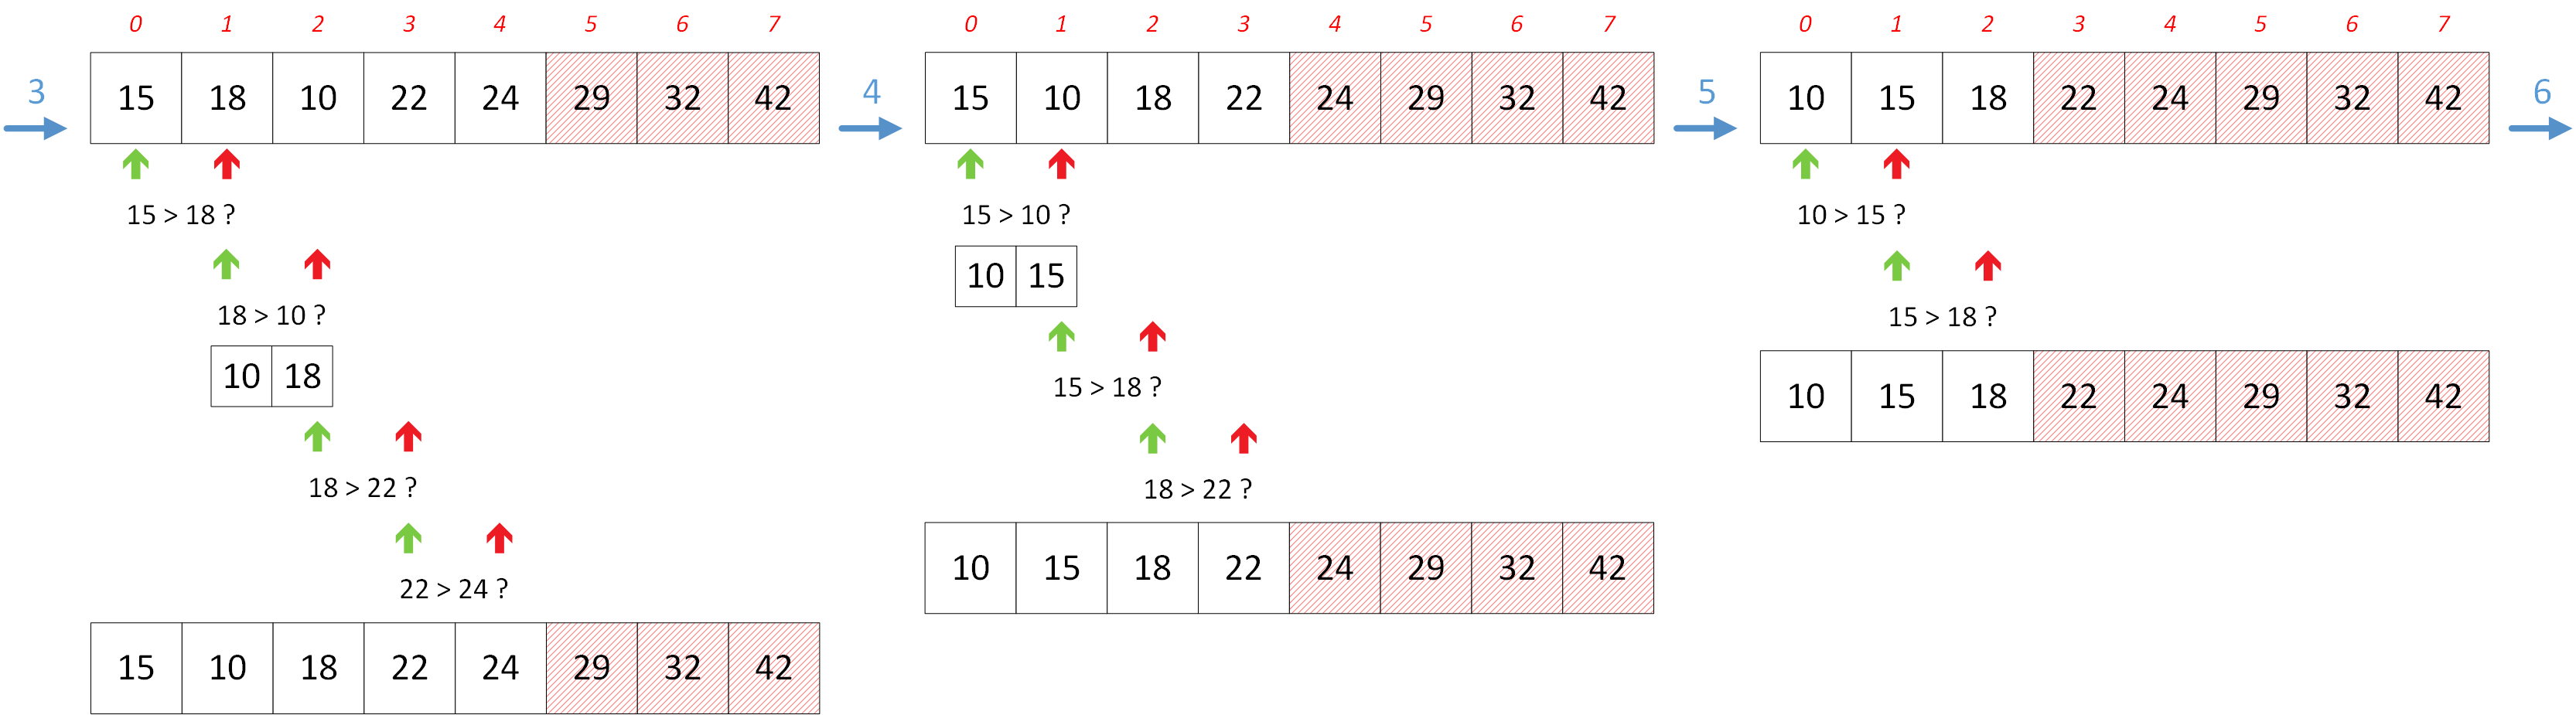
\includegraphics[width=1.2\textwidth]{img/BubbleSort_part2_1.png}
}
%\caption{Bubble Sort part 1}
%\label{figure:1-S3-DesignScience-ThreeLoops}
\end{figure}
%\end{figure*} % Figure flottante
% To use it : fig~\ref{label}


%\begin{figure*} % Figure flottante
\begin{figure}[ht!]
\centering
\centerline{
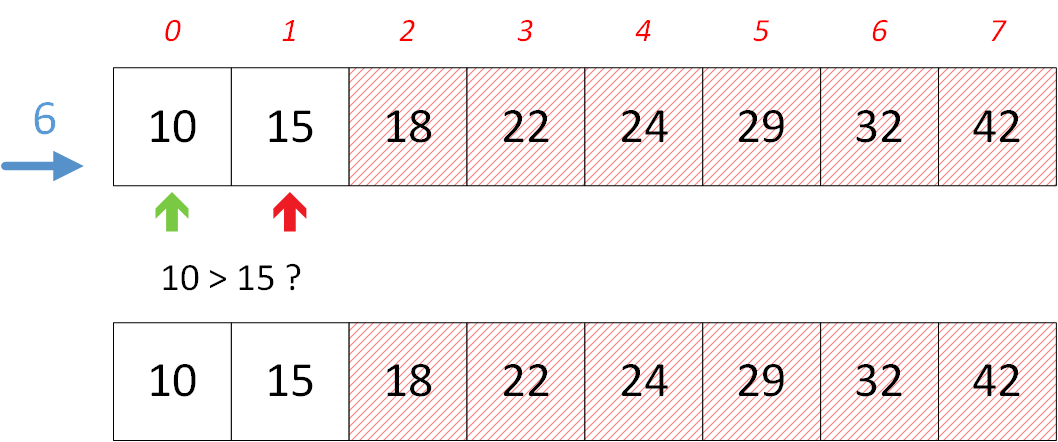
\includegraphics[scale=0.48]{img/BubbleSort_part2_2.png}
}
%\caption{Bubble Sort part 1}
%\label{figure:1-S3-DesignScience-ThreeLoops}
\end{figure}
%\end{figure*} % Figure flottante
% To use it : fig~\ref{label}

\bigskip

\question{Écrivez une procédure de tri respectant l'algorithme du tri à bulles (ou \textit{bubble sort} en anglais). Vous devez modifier la position des éléments dans le tableau créer de tableau supplémentaire. \textit{BubbleSort(tab, len)} }

\vfillLast

%\bigskip
\clearpage


\subsection{Tri par sélection}

\medskip

Le tri par sélection est le tri le plus évident humainement parlant : on cherche le plus grand élément dans le tableau en parcourant toutes les cases, puis, on échange la place de cet élément avec le tout dernier du tableau (pour le placer à sa place définitive).
On recommence ce traitement (sans lire la dernière case à chaque fois) jusqu'à avoir ordonné tous les éléments.

\vfillFirst

%\begin{figure*} % Figure flottante
\begin{figure}[ht!]
\centering
\centerline{
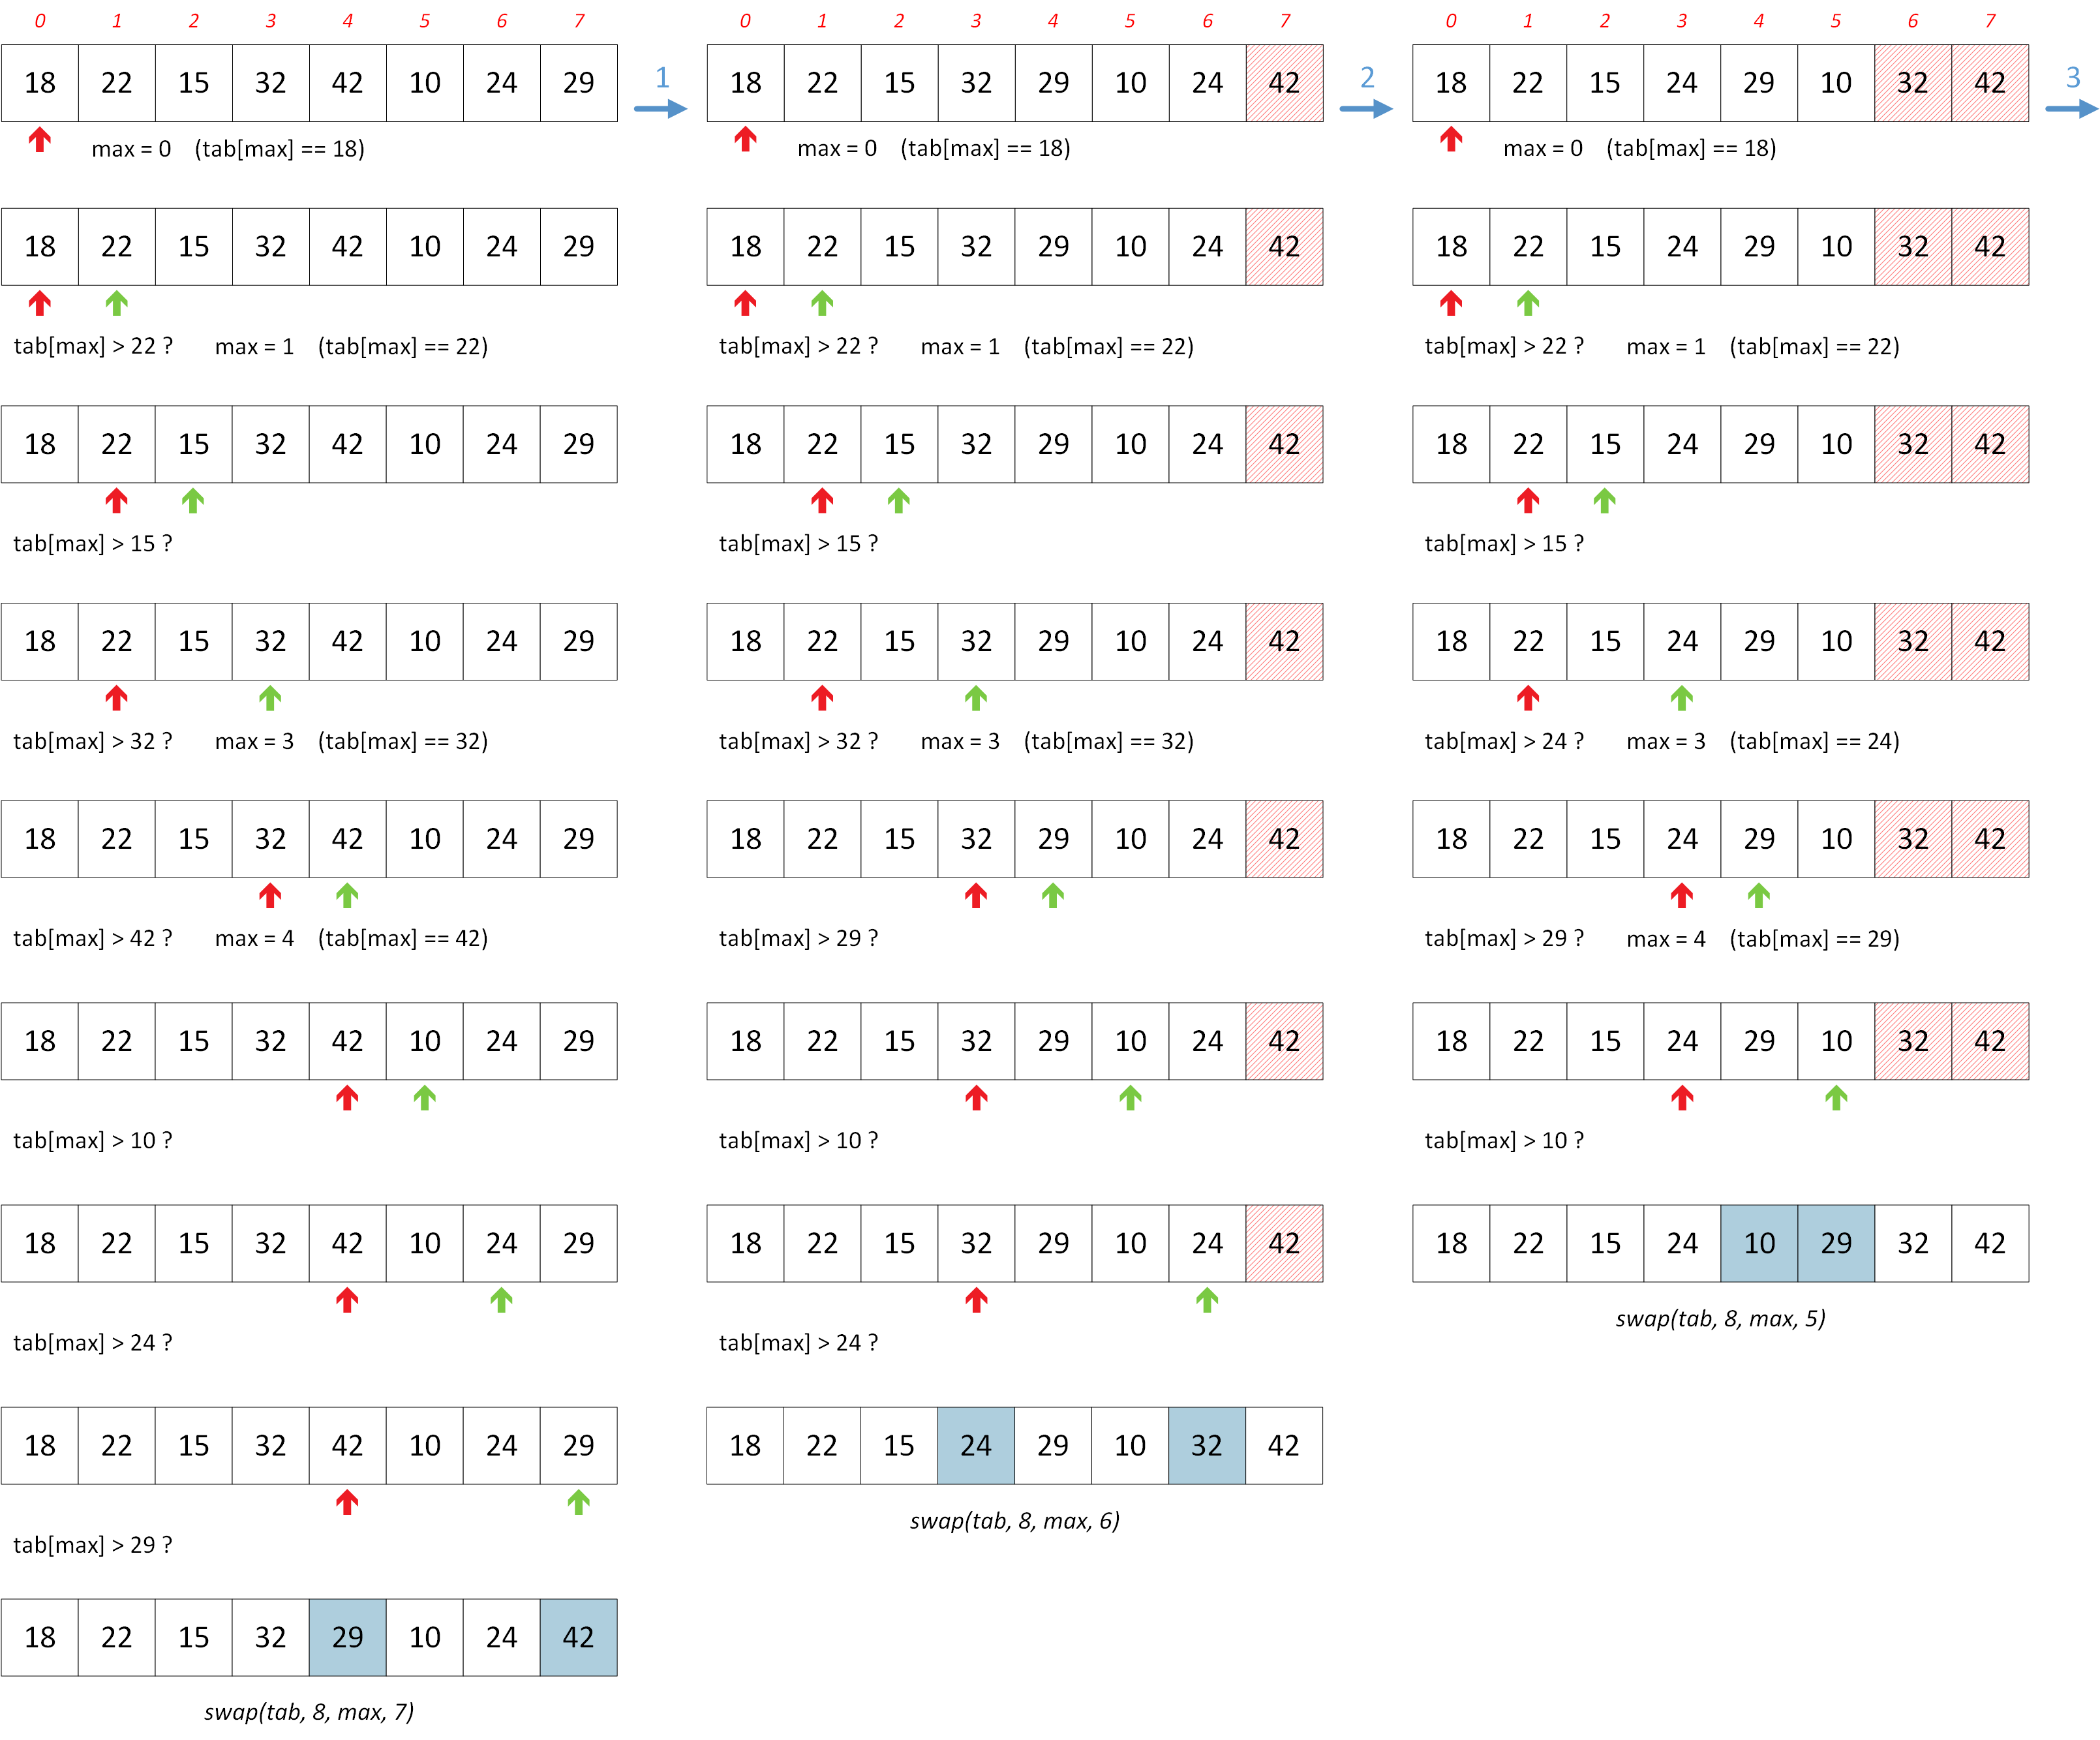
\includegraphics[width=1.2\textwidth]{img/SelectionSort_part1.png}
}
%\caption{Bubble Sort part 1}
%\label{figure:1-S3-DesignScience-ThreeLoops}
\end{figure}
%\end{figure*} % Figure flottante
% To use it : fig~\ref{label}

\vfillLast

\clearpage

\vfillFirst

%\begin{figure*} % Figure flottante
\begin{figure}[ht!]
\centering
\centerline{
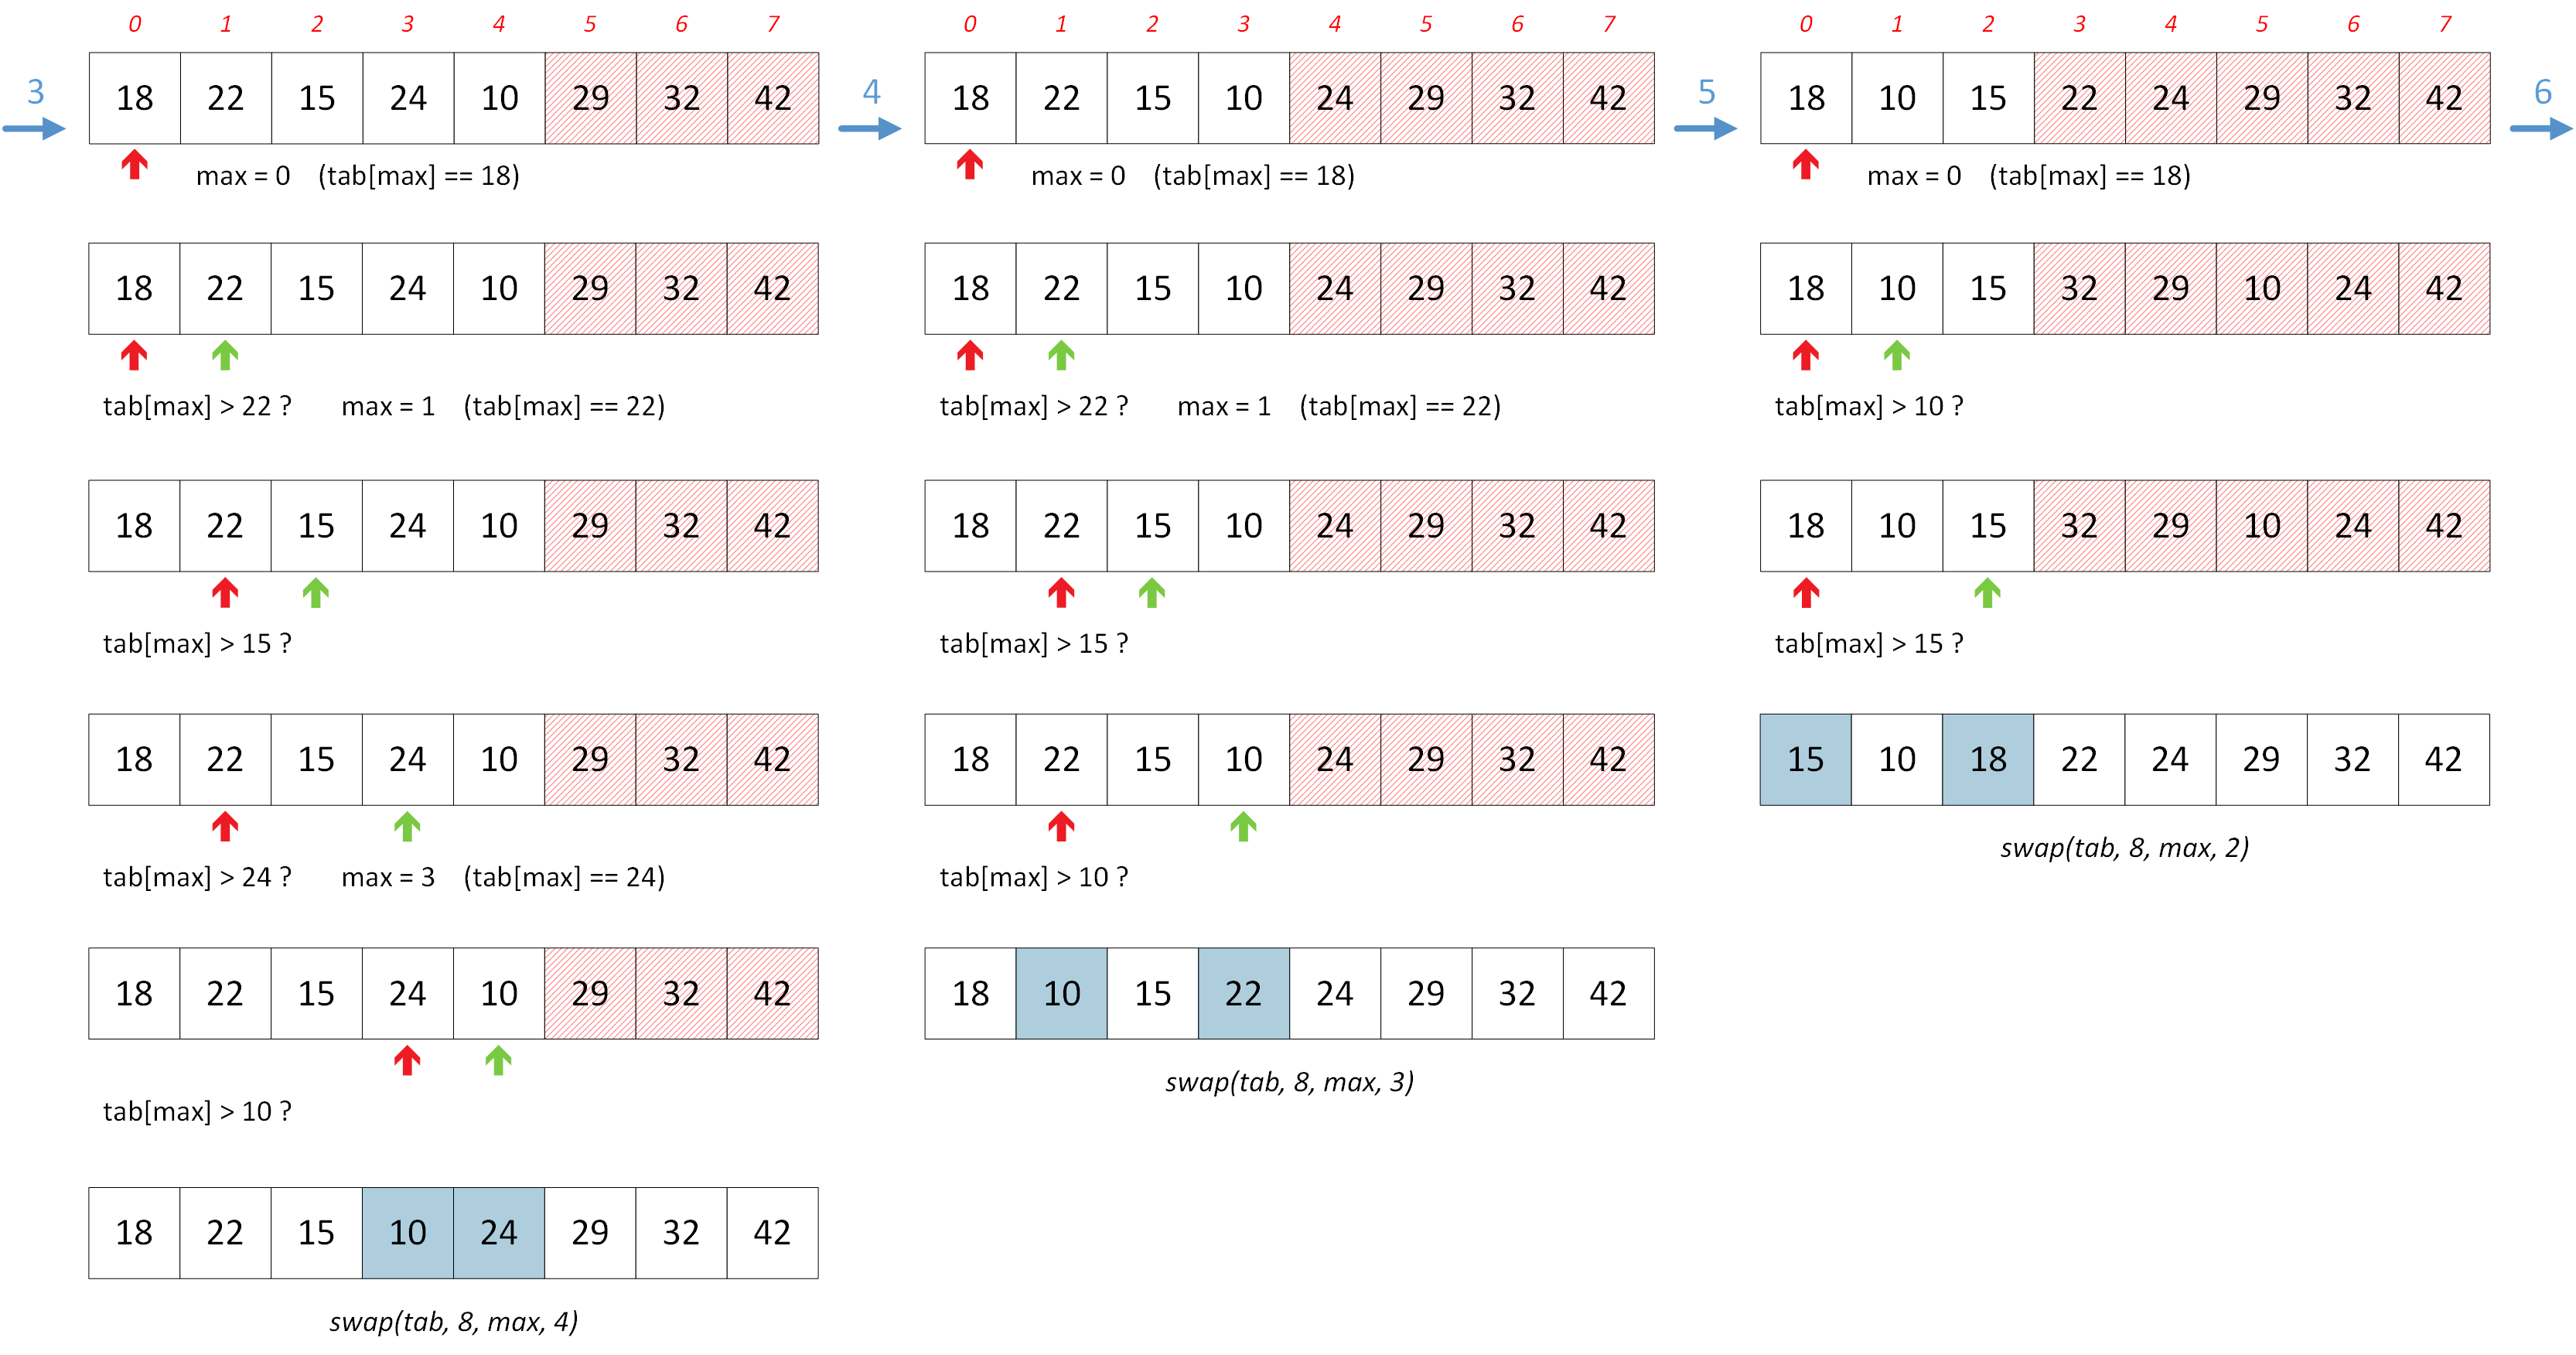
\includegraphics[width=1.2\textwidth]{img/SelectionSort_part2_1.png}
}
%\caption{Bubble Sort part 1}
%\label{figure:1-S3-DesignScience-ThreeLoops}
\end{figure}
%\end{figure*} % Figure flottante
% To use it : fig~\ref{label}

%\begin{figure*} % Figure flottante
\begin{figure}[ht!]
\centering
\centerline{
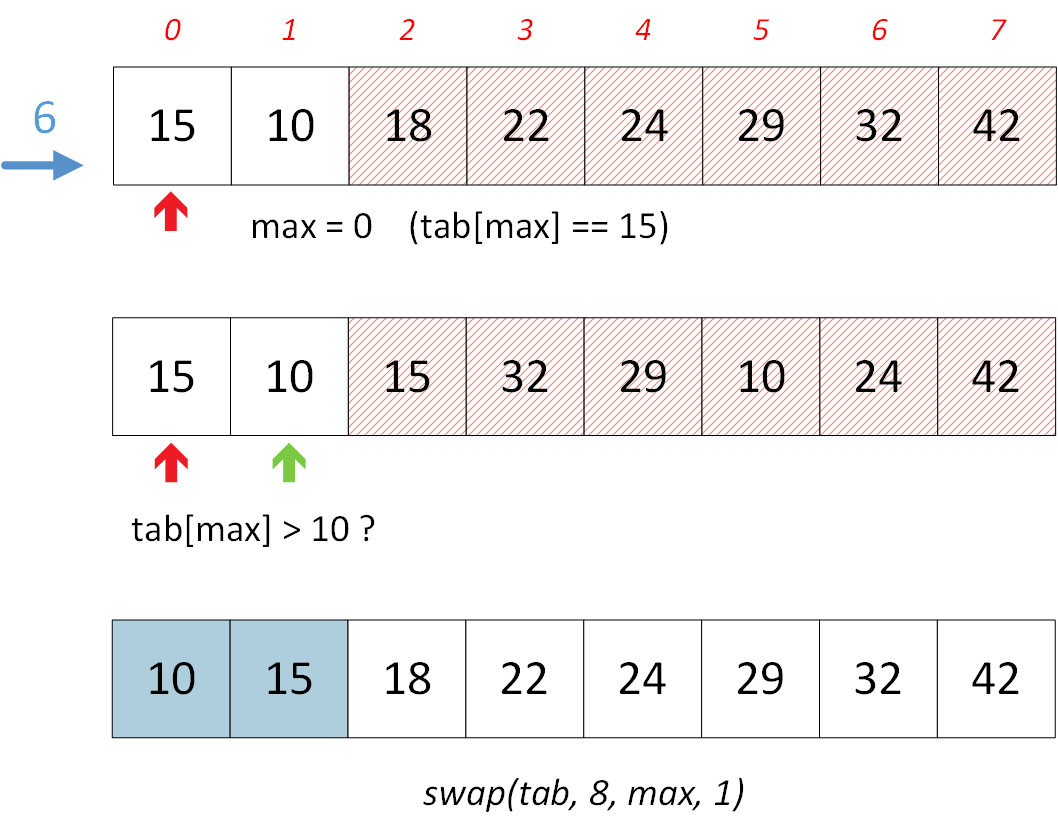
\includegraphics[scale=0.5]{img/SelectionSort_part2_2.png}
}
%\caption{Bubble Sort part 1}
%\label{figure:1-S3-DesignScience-ThreeLoops}
\end{figure}
%\end{figure*} % Figure flottante
% To use it : fig~\ref{label}

\bigskip

\question{Écrivez une procédure de tri respectant l'algorithme du tri par sélection (ou \textit{selection sort} en anglais). Vous devez modifier la position des éléments dans le tableau sans créer de tableau supplémentaire. \textit{SelectionSort(tab, len)} }

\vfillLast

\clearpage

\subsection{Tri par insertion}

Le tri par insertion considère que le tableau donné en paramètre n'est pas trié, et seuls les éléments qu'il a manipulé successivement le sont.
Ainsi, chaque élément du tableau est comparé à tous ceux déjà triés, et on le place là où il devrait être.
Pour le premier élément, celui-ci est considéré comme déjà trié, on peut donc passer au deuxième.
Le deuxième est comparé avec l'unique élément déjà trié : on échange leurs deux places si nécessaire.
Le troisième élément est comparé au plus grand des deux éléments triés, s'il est plus grand ou égal, il reste à sa place, sinon on le décale vers la gauche d'un cran, et on le compare à l'élément suivant (et ainsi de suite).
Chaque élément du tableau est donc \textit{inséré} à sa place parmi les éléments considérés comme triés.

%\begin{figure*} % Figure flottante
\begin{figure}[ht!]
\centering
\centerline{
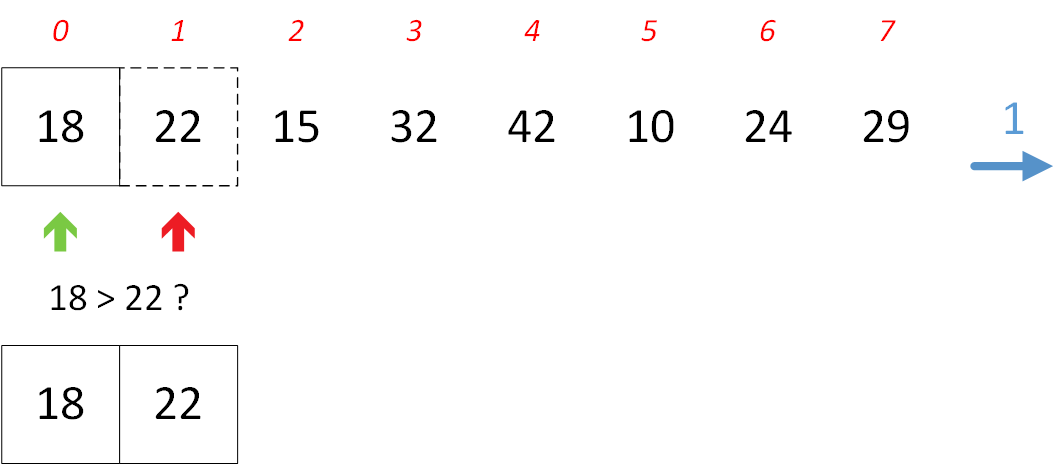
\includegraphics[scale=0.48]{img/InsertionSort_part1_1.png}
}
%\caption{Bubble Sort part 1}
%\label{figure:1-S3-DesignScience-ThreeLoops}
\end{figure}
%\end{figure*} % Figure flottante
% To use it : fig~\ref{label}

%\begin{figure*} % Figure flottante
\begin{figure}[ht!]
\centering
\centerline{
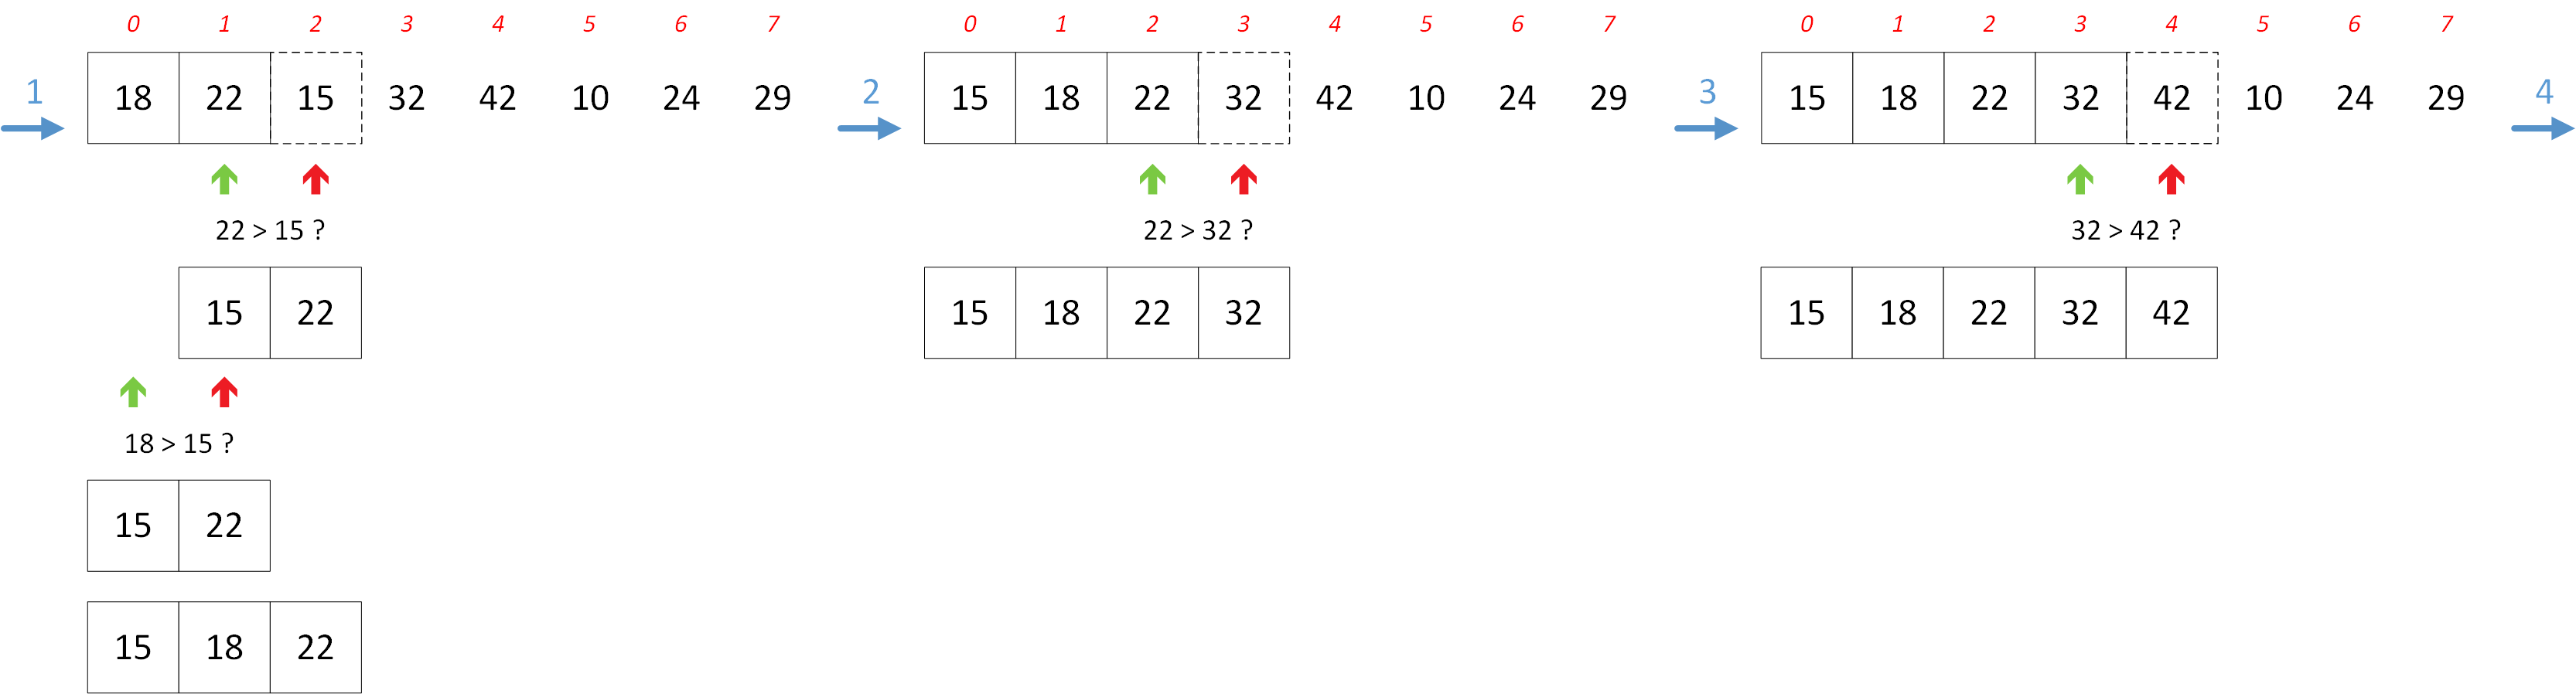
\includegraphics[width=1.18\textwidth]{img/InsertionSort_part1_2.png}
}
%\caption{Bubble Sort part 1}
%\label{figure:1-S3-DesignScience-ThreeLoops}
\end{figure}
%\end{figure*} % Figure flottante
% To use it : fig~\ref{label}

%\begin{figure*} % Figure flottante
\begin{figure}[ht!]
\centering
\centerline{
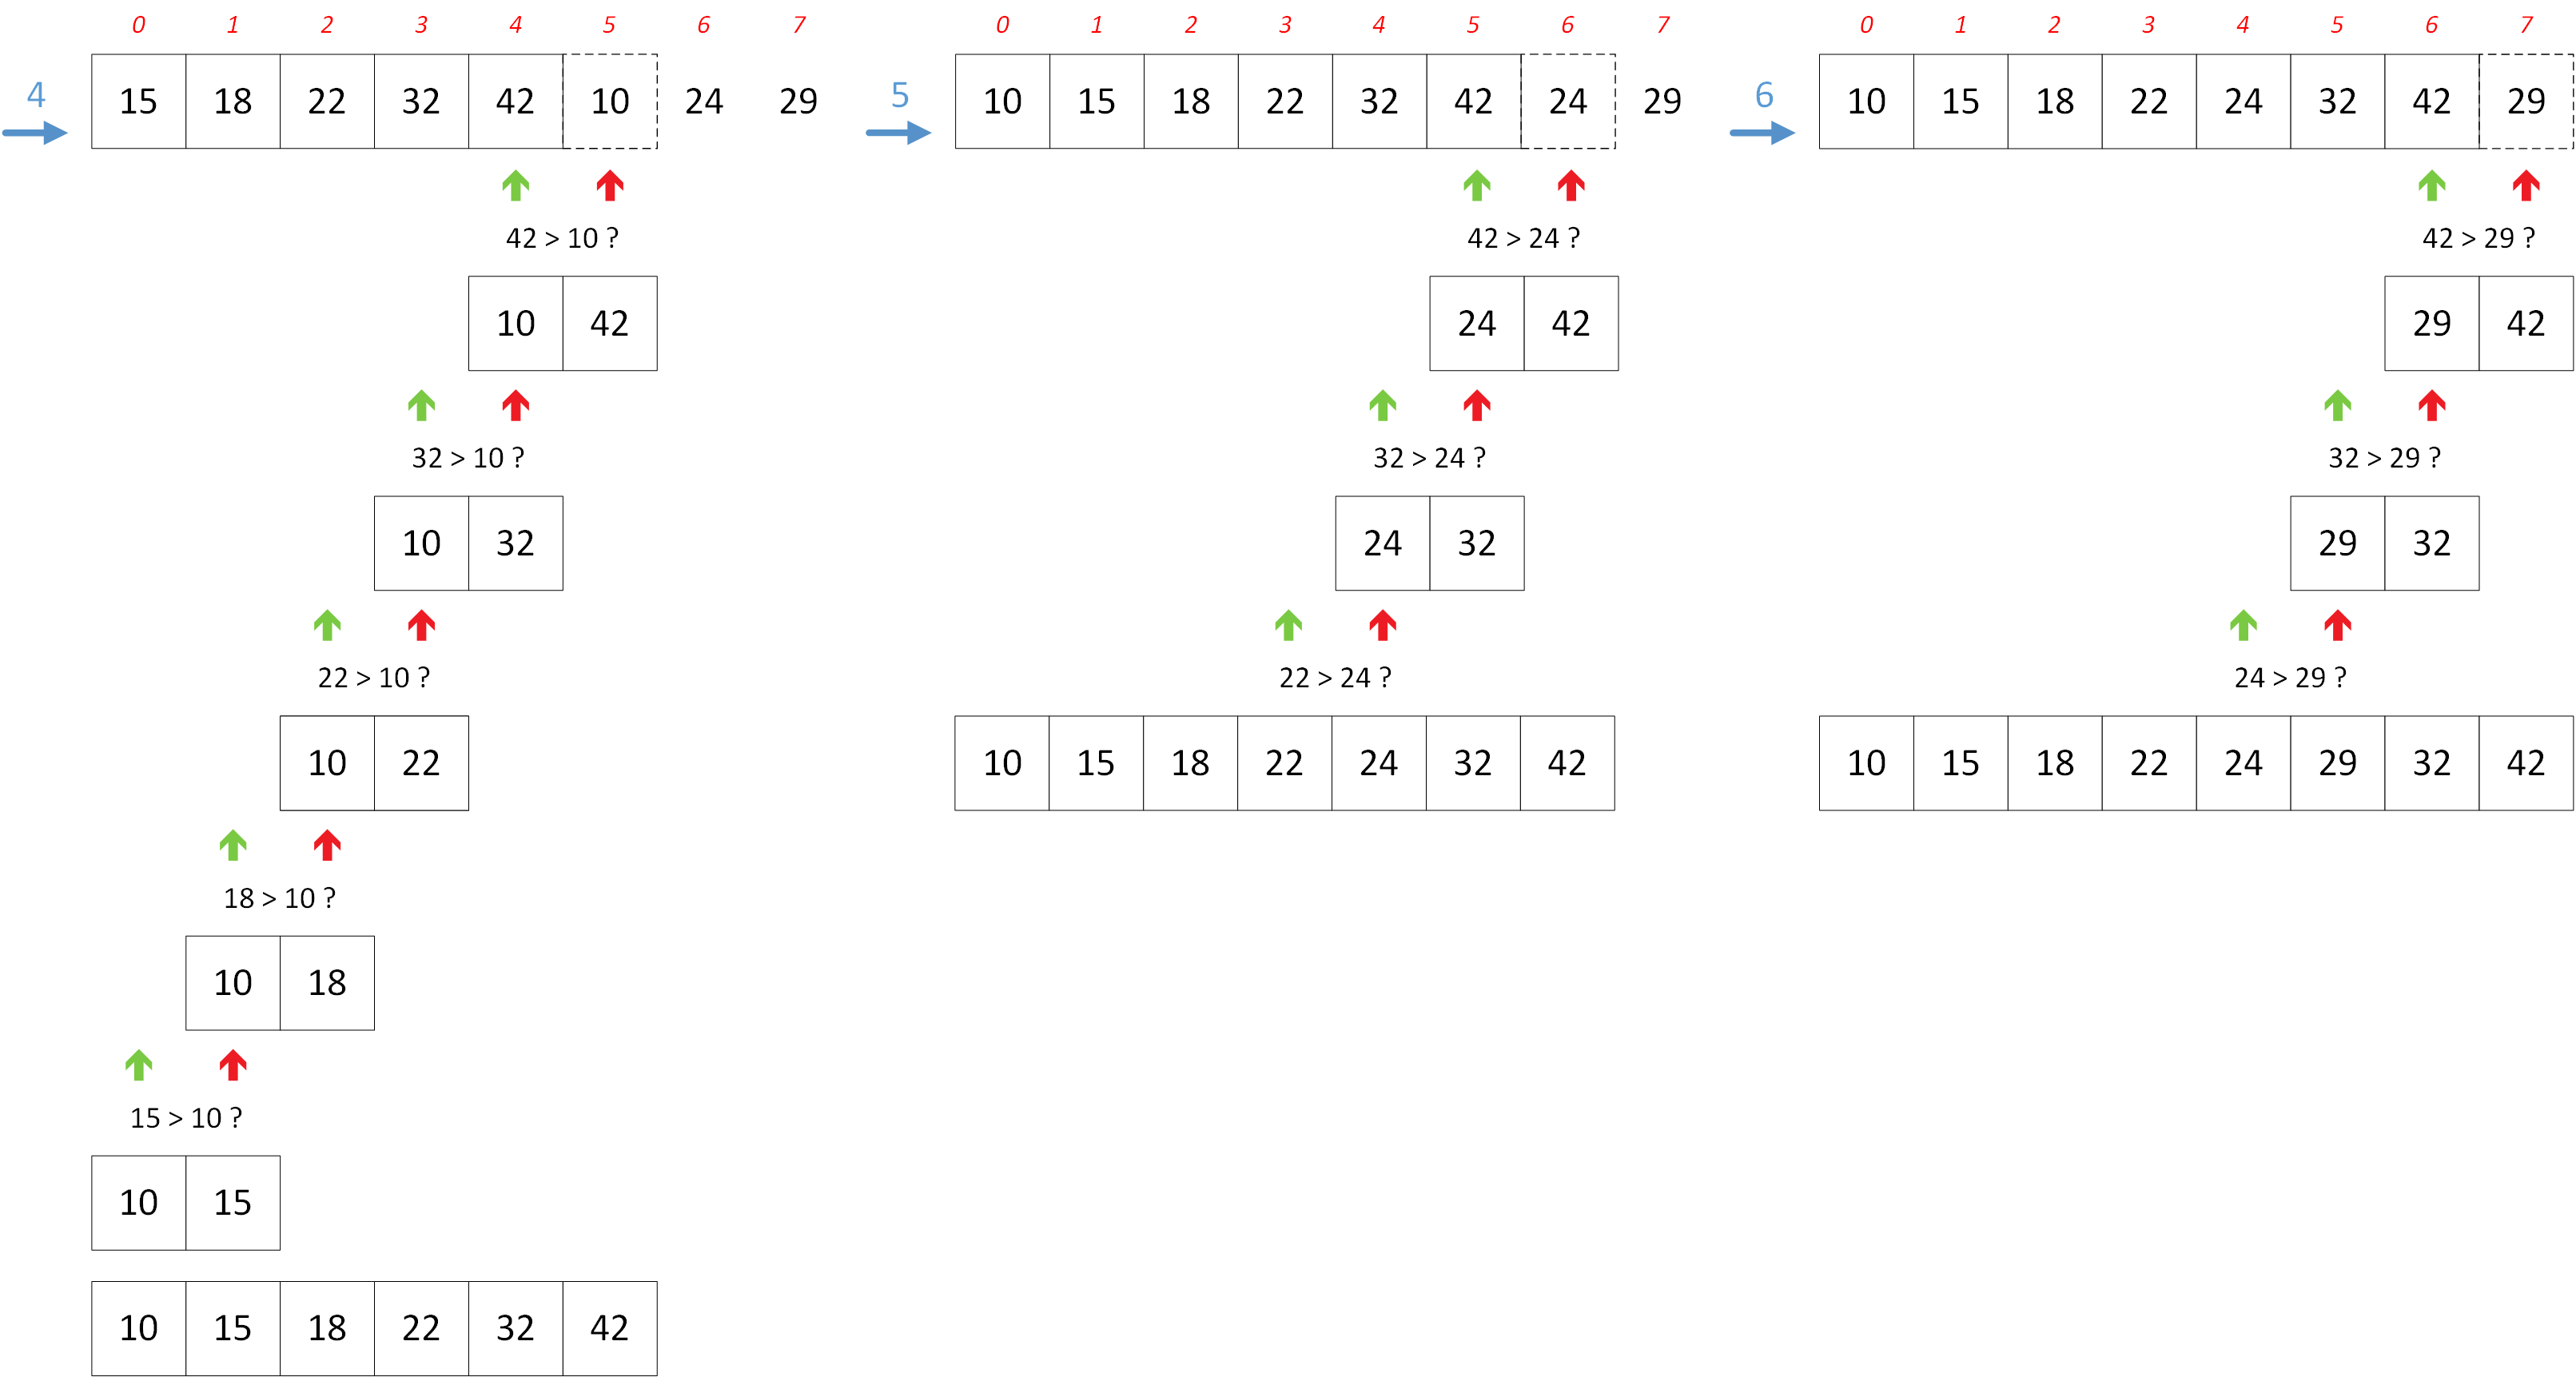
\includegraphics[width=1.18\textwidth]{img/InsertionSort_part2.png}
}
%\caption{Bubble Sort part 1}
%\label{figure:1-S3-DesignScience-ThreeLoops}
\end{figure}
%\end{figure*} % Figure flottante
% To use it : fig~\ref{label}

%\bigskip
\clearpage

\question{Écrivez une procédure de tri respectant l'algorithme du tri par insertion (ou \textit{insertion sort} en anglais). Vous devez modifier la position des éléments dans le tableau créer de tableau supplémentaire. \textit{InsertionSort(tab, len)} }



\vfillFirst

\vfillLast


\begin{center}
\textit{Ce document et ses illustrations ont été réalisés par Fabrice BOISSIER en octobre 2022.\\
La plupart des exercices sont inspirés du cahier d'algo de Nathalie "Junior" BOUQUET et Christophe "Krisboul" BOULLAY.}
\end{center}

\end{document}
